\documentclass[10pt,a4paper]{article}


\addtolength{\oddsidemargin}{-.5in}
\addtolength{\evensidemargin}{-.5in}
\addtolength{\textwidth}{1in}
\addtolength{\topmargin}{-.5in}
\addtolength{\textheight}{1in}

\usepackage{color}
\usepackage{booktabs}
\usepackage{colortbl}
\usepackage[utf8]{inputenc}
\usepackage{caption}
\usepackage{graphics}
\usepackage{graphicx}
\usepackage{float}
\usepackage{xcolor}
\usepackage{subcaption}
\usepackage{lipsum}
\usepackage{hyperref}
\usepackage{multirow}
\usepackage{multicol}
\usepackage{booktabs}
\graphicspath{{figures/}}
\usepackage{imakeidx}
\makeindex

\begin{document}
\title{Hepatitis C Virus Prediction \\ 
\Large{Report per l'Esame di Fondamenti di Machine Learning}}
\author{\textsc{Filippo Casari}\\
    \emph{matr. 132591} \\
    Ingegneria Informatica\\
    \emph{256034@studenti.unimore.it}
    }
\date{}


\maketitle
% Abstract
\clearpage
\tableofcontents{}
\clearpage

\begin{abstract}

\normalsize
Si stima che nel Mondo ci siano tra i 130 e 170 milioni di individui affetti da epatite C e che solo nel 15\% dei casi si possa effettivamente arrivare ad una risoluzione medica. Scopo di questo progetto è analizzare un dataset contenete dati di oltre 1300 pazienti egiziani infetti e, attraverso algoritmi di Machine Learning, tra i quali i metodi di classificazione multiclasse K-Nearest Neighbors e Decision Tree, cercare di trovare dei modelli tali da poter prevedere per un nuovo paziente la dignosi dello stadio della malattia senza ricorrere come ora a metodi clinici invasivi. I livelli per stimare la gravità della malattia sono stati classificati attravero 4 classi. 


\end{abstract}


\section{Introduzione}\label{sec:Introduction}
L'obbiettivo di questa introduzione è quella di fornire un quadro generale del problema dell'HCV e della descrizione dei dati raccolti.
\subsection{Contestualizzazione}\label{ssec:Context}

L'epatite C è un fenomeno altamente presente in Egitto poichè vi è stata una campagna di massa per la diagnosi di schistosomiasi in cui sono state utilizzate delle siringhe impropriamente sterilizzate. Questo tipo di malattia colpisce il fegato ed è estremamente difficile da rilevare poichè il più delle volte è asintomatico nei primi decenni. Tuttavia, i pazienti i cui dati sono stati riportati nel dataset, hanno una qualche forma di fibrosi e sono stati sottoposti ad un trattamento medico.
\subsection{Descrizione delle features raccolte}

La diagnosi dell'HCV può avvenire attraverso diversi metodi e, da qui, la scelta di avere determinati dati riguardanti i pazienti sottoposti ad un trattamento medico. Infatti le infezioni vengono scoperte grazie a indagini riguardanti elevati livelli di enzimi epatici tra i quali l'analina transaminasi (\textbf{ALT}) e l'aspartate transaminase (\textbf{ASP}). L'ALT è stato analizzato per ogni paziente dopo \textit{1, 4, 12, 24, 32 e 64} settimane durante il trattamento per l'HCV per monitorare il paziente stesso. Un altro fattore chiave è stato quello di rilevare l'RNA che contraddistingue il virus, monitorando questo valore fin dall'inizio (\textbf{RNA base}), a 4 e a 12 settimane dall'inizio del trattamento e alla fine (\textbf{RNA EOF}, end-of-treatment). Effettivamente dopo 12 settimane se il valore di RNA del virus dovesse essere molto alto, vorrebbe dire che il paziente è afflitto da una cirrosi cronica. Oltre a questi fattori, sono stati inclusi nel dataset: \textit{età, genere, indice di massa corporea (BMI), febbre, Nausea, mal di testa, diarrea, stanchezza e dolori alle ossa, ittero, piastrine, dolore epigastrero e i livelli di emoglobina e varie cellule (leucociti, ovvero WBC, e globuli rossi, ovvero RBC)}. Nel dataset sono presenti altri valori potenzialmente rilevanti ai fini della classificazione come il \textbf{Baseline histological Grading} ottenuto tramite biopsie epatiche per determinare il grado di danno del fegato. Come menzionato precedentemente, il target value è sicuramente lo stadio di fibrosi che affligge il paziente, ovvero il Baselinehistological staging che è stato classificato attraverso 4 valori, dal meno grave al più grave: \textbf{portal fibrosis, few septa, many septa e cirrhosis}.
\newline Le librerie python utilizzate sono state: NumPy, Pandas, Sklearn, Matplot e SeaBorn.\cite{sklearn}



\clearpage
% RNA base ==> scartato poichè c'è solo una classe
\section{Analisi dei dati}\label{sec:analisi_dati}\cite{LEZIONI}

In questa sezione avviene l'esplorazione del dataset completo, considerando diverse caratteristiche tra le quali:
\begin{itemize}
\item Ricerca di eventuali valori nulli
\item Ricerca di eventuali valori mancanti
\item valori discreti o continui
\item Tipo di dati
\item Range delle features
\item collinearità, multicollinearità dei dati
\item matrice di correlazione





\end{itemize}
\subsection{EDA: Exploratory Data Analysis}\label{ssec:EDA}

Il dataset è composto da 28 features metre, come mezionato precedentemente, la target label è stata classificata in 4 classi da un team di medici egiziani. Sono stati campionati in tutto 1385 samples, ogni sample contiene i dati del paziente.
Per avere un'informazione dettagliata e precisa dei dati sono state impigate le funzioni di pandas tra le quali: pandas.describe() e pandas.info(). Tutte e due le funzioni prendono in input il dataset completo e mentre la prima descrive la tipologia dei dati e il conteggio di essi, la seconda dà inforazioni riguardanti diversi ulteriori parametri come la media per ogni features, il minimo, il massimo valore e i percentili.  
Analizzando il dataset attraverso questi metodi, non ci sono valori nulli/mancanti nè feature duplicate e i tipi di dati sono int e float. 


\begin{table}[ht]
\centering
\begin{tabular}{|l|l|l|l|l|} 
\hline
\rowcolor{black}                                            & \textcolor{white}{\textbf{\textit{RNA EOT}}} & \textcolor{white}{\textbf{\textit{RNA 12}}} & \begin{tabular}[c]{@{}>{\cellcolor{black}}l@{}}\textcolor{white}{\textbf{Baseline histological }}\\\textcolor{white}{\textbf{Grading}}\end{tabular} & \begin{tabular}[c]{@{}>{\cellcolor{black}}l@{}}\textcolor{white}{\textbf{\textit{Baseline histological }}}\\\textcolor{white}{\textbf{\textit{Grading}}}\end{tabular}  \\ 
\hline
\rowcolor{black} \textcolor{white}{\textbf{\textit{count}}} & \textcolor{white}{\textbf{1385}}             & \textcolor{white}{\textbf{1385}}            & \textcolor{white}{\textbf{1385}}                                                                                                                    & \textcolor{white}{\textbf{1385}}                                                                                                                                       \\ 
\hline
\rowcolor{black} \textcolor{white}{\textbf{\textit{mean}}}  & \textcolor{white}{\textbf{287660.336462}}    & \textcolor{white}{\textbf{2.887536e+05}}    & \textcolor{white}{\textbf{~9.761733~}}                                                                                                              & \textcolor{white}{\textbf{2.536462}}                                                                                                                                   \\ 
\hline
\rowcolor{black} \textcolor{white}{\textbf{\textit{std}}}   & \textcolor{white}{\textbf{264559.525070}}    & \textcolor{white}{\textbf{2.853507e+05}}    & \textcolor{white}{\textbf{4.023896}}                                                                                                                & \textcolor{white}{\textbf{1.121392}}                                                                                                                                   \\ 
\hline
\rowcolor{black} \textcolor{white}{\textbf{\textit{min}}}   & \textcolor{white}{\textbf{5}}                & \textcolor{white}{\textbf{5}}               & \textcolor{white}{\textbf{3}}                                                                                                                       & \textcolor{white}{\textbf{1}}                                                                                                                                          \\ 
\hline
\rowcolor{black} \textcolor{white}{\textbf{\textit{25\%}}}  & \textcolor{white}{\textbf{5}}                & \textcolor{white}{\textbf{5}}               & \textcolor{white}{\textbf{6}}                                                                                                                       & \textcolor{white}{\textbf{2}}                                                                                                                                          \\ 
\hline
\rowcolor{black} \textcolor{white}{\textbf{\textit{50\%}}}  & \textcolor{white}{\textbf{251376}}           & \textcolor{white}{\textbf{2.343590e+05}}    & \textcolor{white}{\textbf{10}}                                                                                                                      & \textcolor{white}{\textbf{3}}                                                                                                                                          \\ 
\hline
\rowcolor{black} \textcolor{white}{\textbf{\textit{75\%}}}  & \textcolor{white}{\textbf{517806}}           & \textcolor{white}{\textbf{5.248190e+05}}    & \textcolor{white}{\textbf{13}}                                                                                                                      & \textcolor{white}{\textbf{4}}                                                                                                                                          \\ 
\hline
\rowcolor{black} \textcolor{white}{\textbf{\textit{max}}}   & \textcolor{white}{\textbf{808450}}           & \textcolor{white}{\textbf{3.731527e+06}}    & \textcolor{white}{\textbf{16}}                                                                                                                      & \textcolor{white}{\textbf{4}}                                                                                                                                          \\
\hline
\end{tabular}
\caption{Alcuni valori estratti da pandas.describe()}
\end{table}

I valori delle features nel caso di RBC, AST, ALT, RNA sono valori continui, mentre alcuni valori come Nausea, Diarrea, Età sono valori discreti. In accordo con le \textbf{raccomandazioni dei medici} mostrate nel dataset description, sono stati \textbf{discretizzati} in dei range ad hoc tutti i valori presenti di ogni feature nel dataset. Questo tipo di operazione, la discretizzazione, è stata effettuta nella fase di EDA e non di preproccessing come normalmente avverrebbe, poichè nella descrizione del dataset si suppone fin dall'inizio di avere il datast già discretizzato. Inoltre, discretizzando i dati, si possono avere dei grafici molto più indicativi dal punto di vista medico dei valori stessi delle features. Sono stati riportati i range delle features per la discretizazione.



\begin{table}[ht]\label{tab:discretization criteria}
\centering
\resizebox{0.7\textwidth}{!}{\begin{minipage}{\textwidth}
\begin{tabular}{lll}
Feature Names                 & Feature Values  & Discretization (Items)                                                                                                                                 \\
Age                           & 32:61           & {[}0; 32], ]32; 37], ]37; 42],]42; 47], ]47; 52], ]52; 57],]57; 62]                                                                                    \\
Gender                        & Male,Female     & {[}Male], [Female]                                                                                                                                     \\
BMI(Body Mass Index)          & 22:35           & {[}0; 18:5[ [18:5; 25[, [25; 30[, [30; 35[, [35; 40[                                                                                                   \\
Fever                         & Absent, Present & {[}Absent], [Present] -                                                                                                                                \\
Nausea/Vomiting               & Absent, Present & {[}Absent], [Present] -                                                                                                                                \\
Headache                      & Absent, Present & {[}Absent], [Present] -                                                                                                                                \\
Diarrhea                      & Absent, Present & {[}Absent], [Present] -                                                                                                                                \\
Fatigue                       & Absent, Present & {[}Absent], [Present] -                                                                                                                                \\
Bone ache                     & Absent, Present & {[}Absent], [Present] -                                                                                                                                \\
Jaundice                      & Absent, Present & {[}Absent], [Present] -                                                                                                                                \\
Epigastria pain               & Absent, Present & {[}Absent], [Present] -                                                                                                                                \\
WBC(White Blood Cells)        & 2991:12101      & {[}0; 4000[, [4000; 11000[, [11000; 12101]                                                                                                             \\
RBC(Red Blood Cells)          & 3816422:5018451 & {[}0; 3000000[, [3000000; 5000000[,[5000000; 5018451]                                                                                                  \\
HGB(Hemoglobin)               & 2:20            & \begin{tabular}[c]{@{}l@{}}If (Gender==[Male]):[2; 14[, [14; 17:5], ]17:5; 20]\\If(Gender==[Female]):[2; 12:3[, [12:3; 15:3], ]15:3; 20]\end{tabular}  \\
Plat(Platelet)                & 93013:226464    & {[}93013; 100000[, [100000; 255000[,[255000; 226465[                                                                                                   \\
AST1(1 week)                  & 0:128     & {[}0; 20[, [20; 40], ]40; 128]                                                                                                                         \\
ALT1(1 week)                  & 0:128      & {[}0; 20[, [20; 40], ]40; 128]                                                                                                                         \\
ALT4(4 weeks)                 & 0:128      & {[}0; 20[, [20; 40], ]40; 128]                                                                                                                         \\
ALT12(12 weeks)               & 0:128      & {[}0; 20[, [20; 40], ]40; 128]                                                                                                                         \\
ALT24(24 weeks)               & 0:128      & {[}0; 20[, [20; 40], ]40; 128]                                                                                                                         \\
ALT36(36 weeks)               & 0:128      & {[}0; 20[, [20; 40], ]40; 128]                                                                                                                         \\
ALT48(48 weeks)               & 0:128      & {[}0; 20[, [20; 40], ]40; 128]                                                                                                                         \\
RNA Base                      & 0:1201086       & {[}0; 5], ]5; 1201086]                                                                                                                                 \\
RNA 4                         & 0:1201715       & {[}0; 5], ]5; 1201715]                                                                                                                                 \\
RNA 12                        & 0:3731527       & {[}0; 5], ]5; 3731527]                                                                                                                                 \\
RNA EOT                       & 0:808450        & {[}0; 5], ]5; 808450]                                                                                                                                  \\
RNA EF(Elongation Factor)     & 0:808450        & {[}0; 5], ]5; 808450]                                                                                                                                  \\
Baseline Histological Grading & 1:16            & {[}1]; [2]; [3]; :::[16]                                                                                                                               \\
                                                     
\end{tabular}\label{tab:tab1}
\end{minipage}}
\caption{\textbf{Criteri di discretizzazione}}
\end{table}

Il dataset risulta essere bilanciato, ovvero ogni classe di fibrosi è presente in modo equamente distribuito. Questa osservazione ci fa precludere un metodo di preprocessing per ribilanciare la fase di addestramento dei modelli. Infatti avere delle classi bilanciate nel dataset farà in modo che il modello impari a distiguere le classi in modo equo, senza dare più importanza ad un tipo di fibrosi rispetto ad un altra.
\begin{figure}[H]
    \centering
    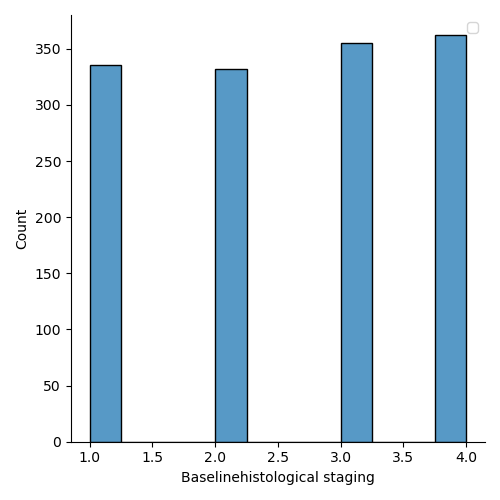
\includegraphics[width=0.5\columnwidth]{figures/target_label.png}
    \caption{Dataset bilanciato}
    \label{fig:target}
\end{figure}



E' stato affrontata l'analisi delle features, dopo la discretizzazione, ed è emerso che alcune feature assumono un solo valore del range stabilito (fig. \ref{fig:distr_features_1}) oppure la maggior parte dei sample ha lo stesso valore, fig. \ref{fig:distr_features_2}. Questo indica che sull'uscita non hanno alcun effetto poichè quello stesso valore compare sempre, indipendentemente dalla classe di output.

\begin{figure}[H]
    \centering
    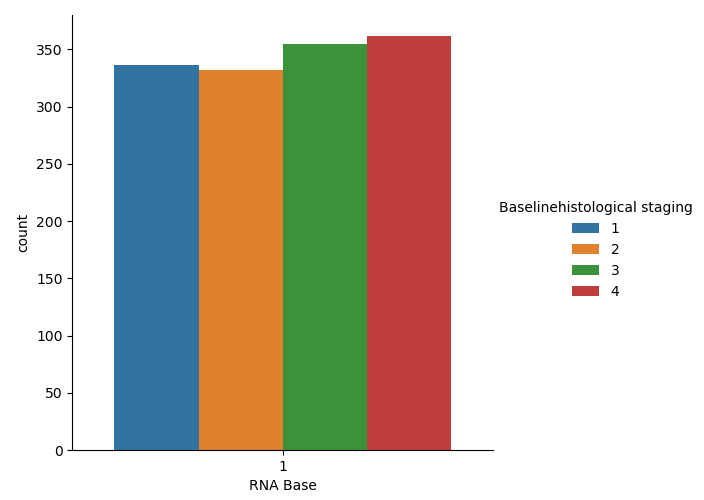
\includegraphics[width=0.4\columnwidth]{figures/RNA base.png}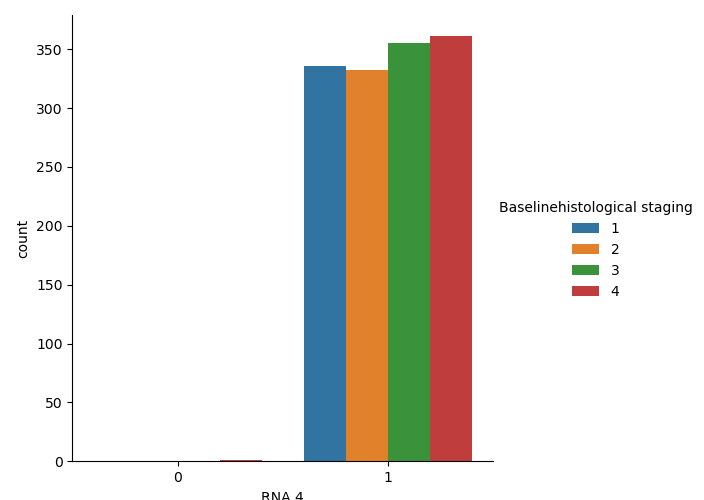
\includegraphics[width=0.4\columnwidth]{figures/RNA 4.png}
    
    \caption{Distribuzione features, un solo valore}
    \label{fig:distr_features_1}
\end{figure}

\begin{figure}[H]
    \centering
    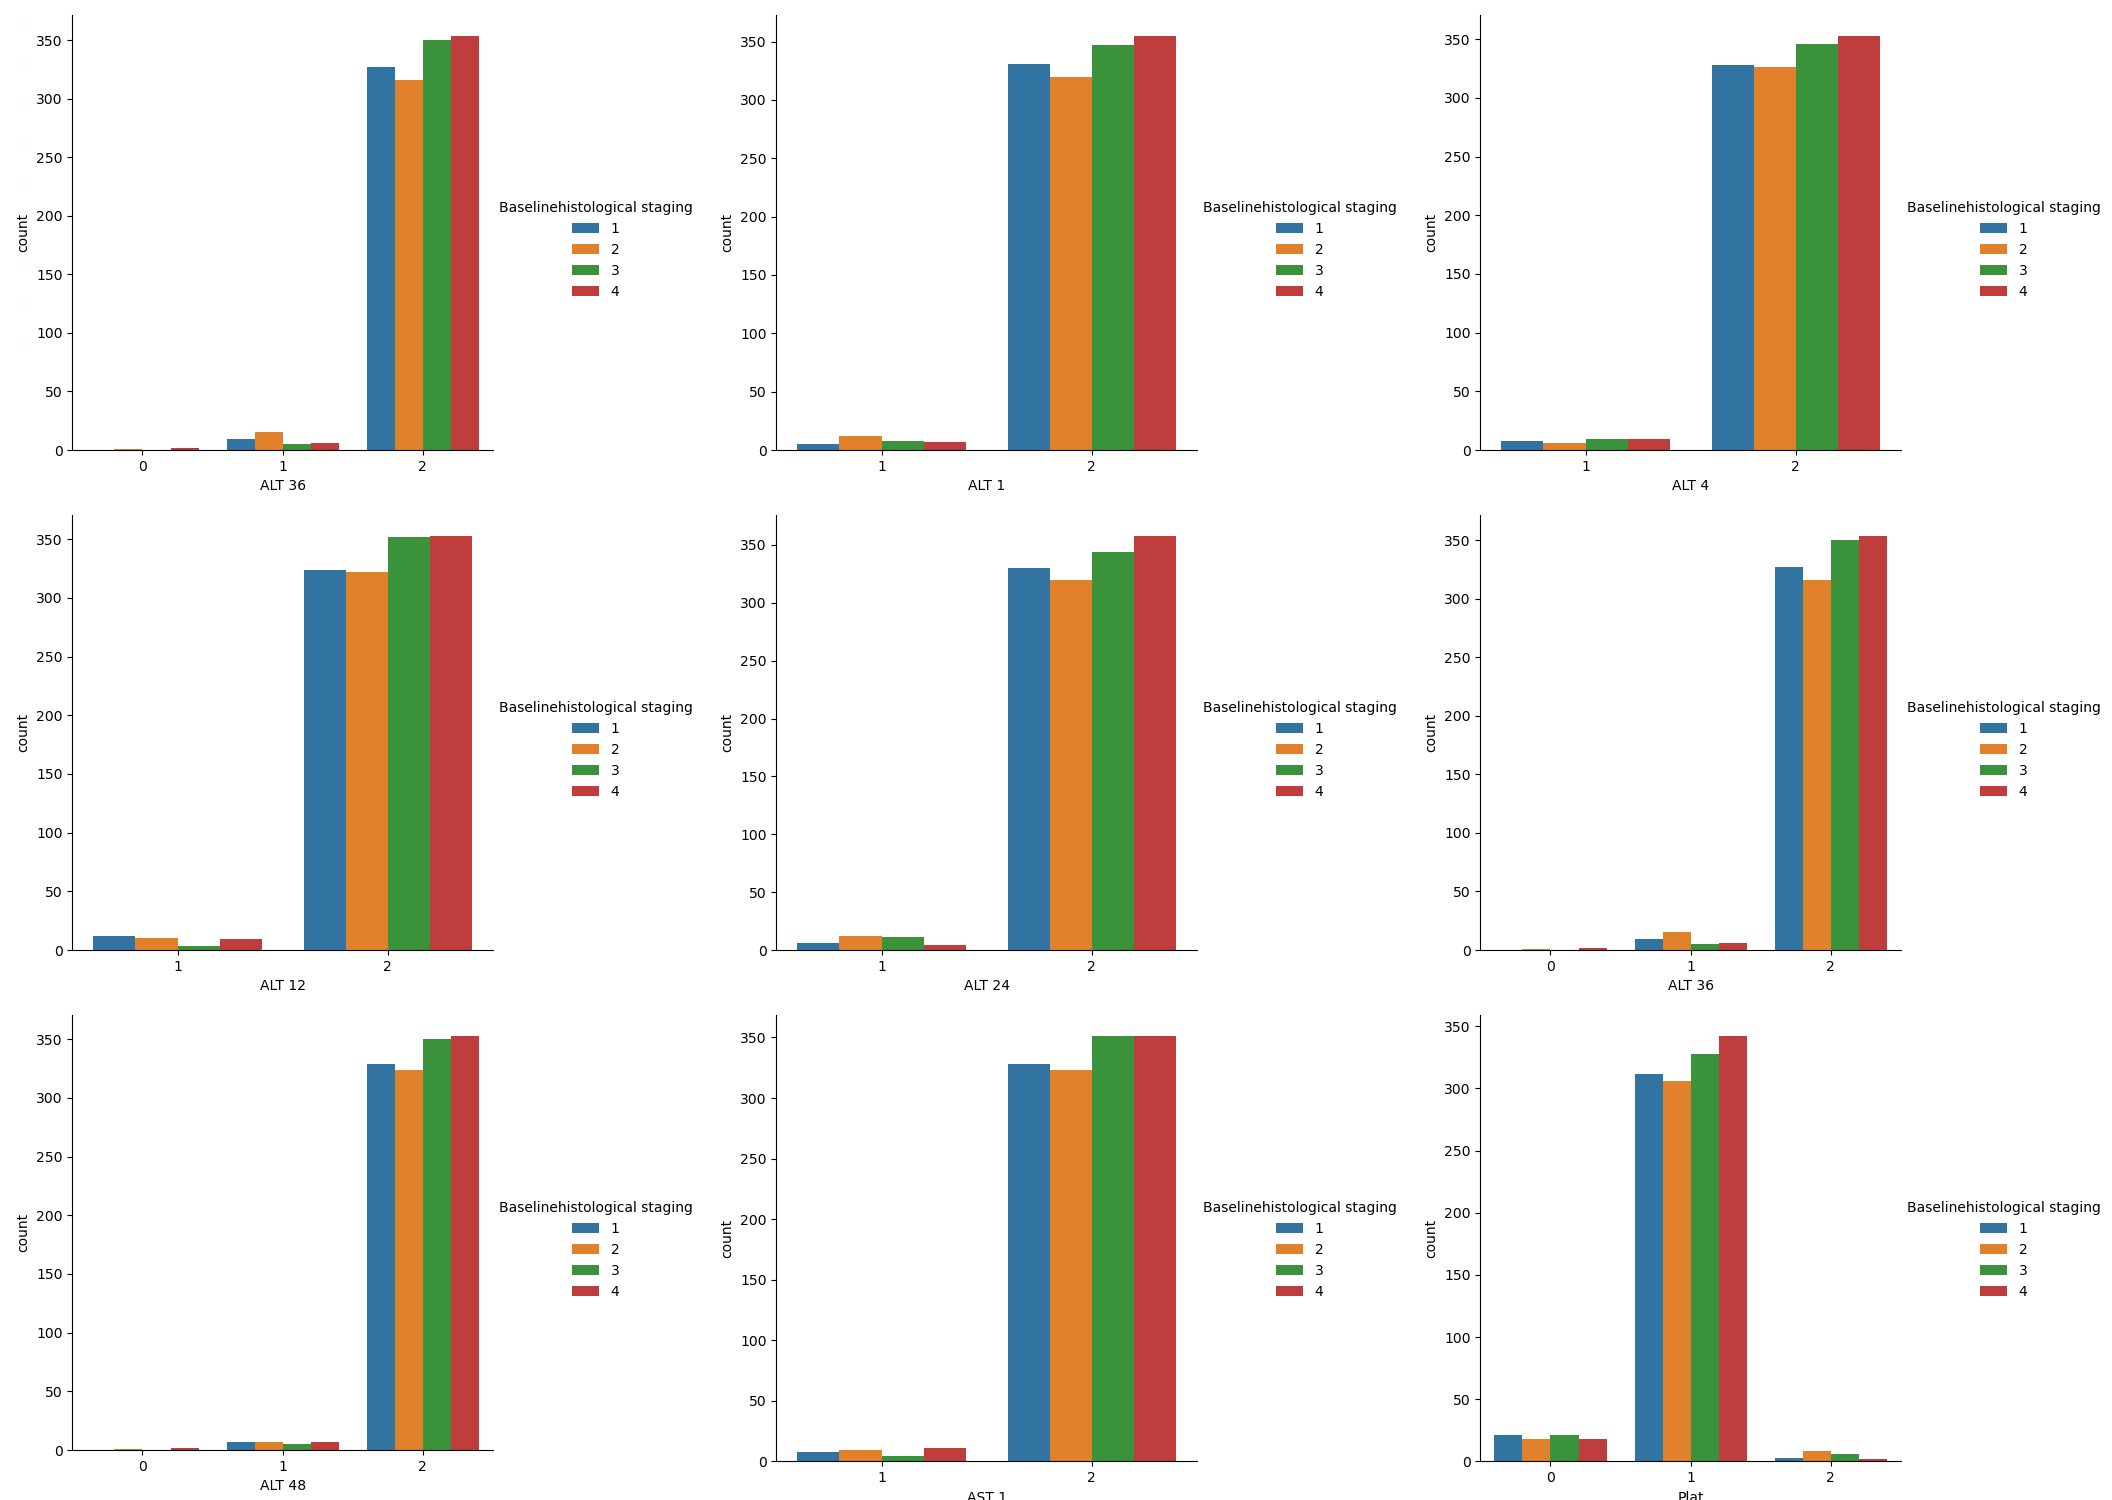
\includegraphics[width=1\columnwidth]{figures/plots_features.png}
    \caption{Distribuzione features, maggior parte dei valori in solo range}
    \label{fig:distr_features_2}
\end{figure}

\subsection{Correlazione tra le features}

Inoltre, il dataset è stato impiegato per valutare la correlazione tra ogni coppia di feature e tra le varie features e l'output target, così da evidenziare eventuali multicollinearità presenti. E' stata usata per questo scopo la matrice di correlazione. Si nota che c'è una discreta correlazione tra le features RNA 12 e RNA EOT. Ciò potrebbe far intuire che i pazienti che hanno l'RNA del virus dopo 12 settimane, probabilmente avranno un indice alto di RNA HCV anche alla fine del trattamento e che quindi sono i più predisposti alla cirrosi cronica. Questa osservazione è in linea con quanto detto precedentemente, ovvero che una volta contratto il virus sarà difficile guarire definitivamente.
Si può notare chiaramente che nessuna delle features è fortemente correlata alla classe target, per cui non c'è collinearità tra l'uscita e le features e, dunque, i metodi migliori per determinare l'output sono quelli di classificazione e non di regressione lineare.

\begin{figure}[H]
    \centering
    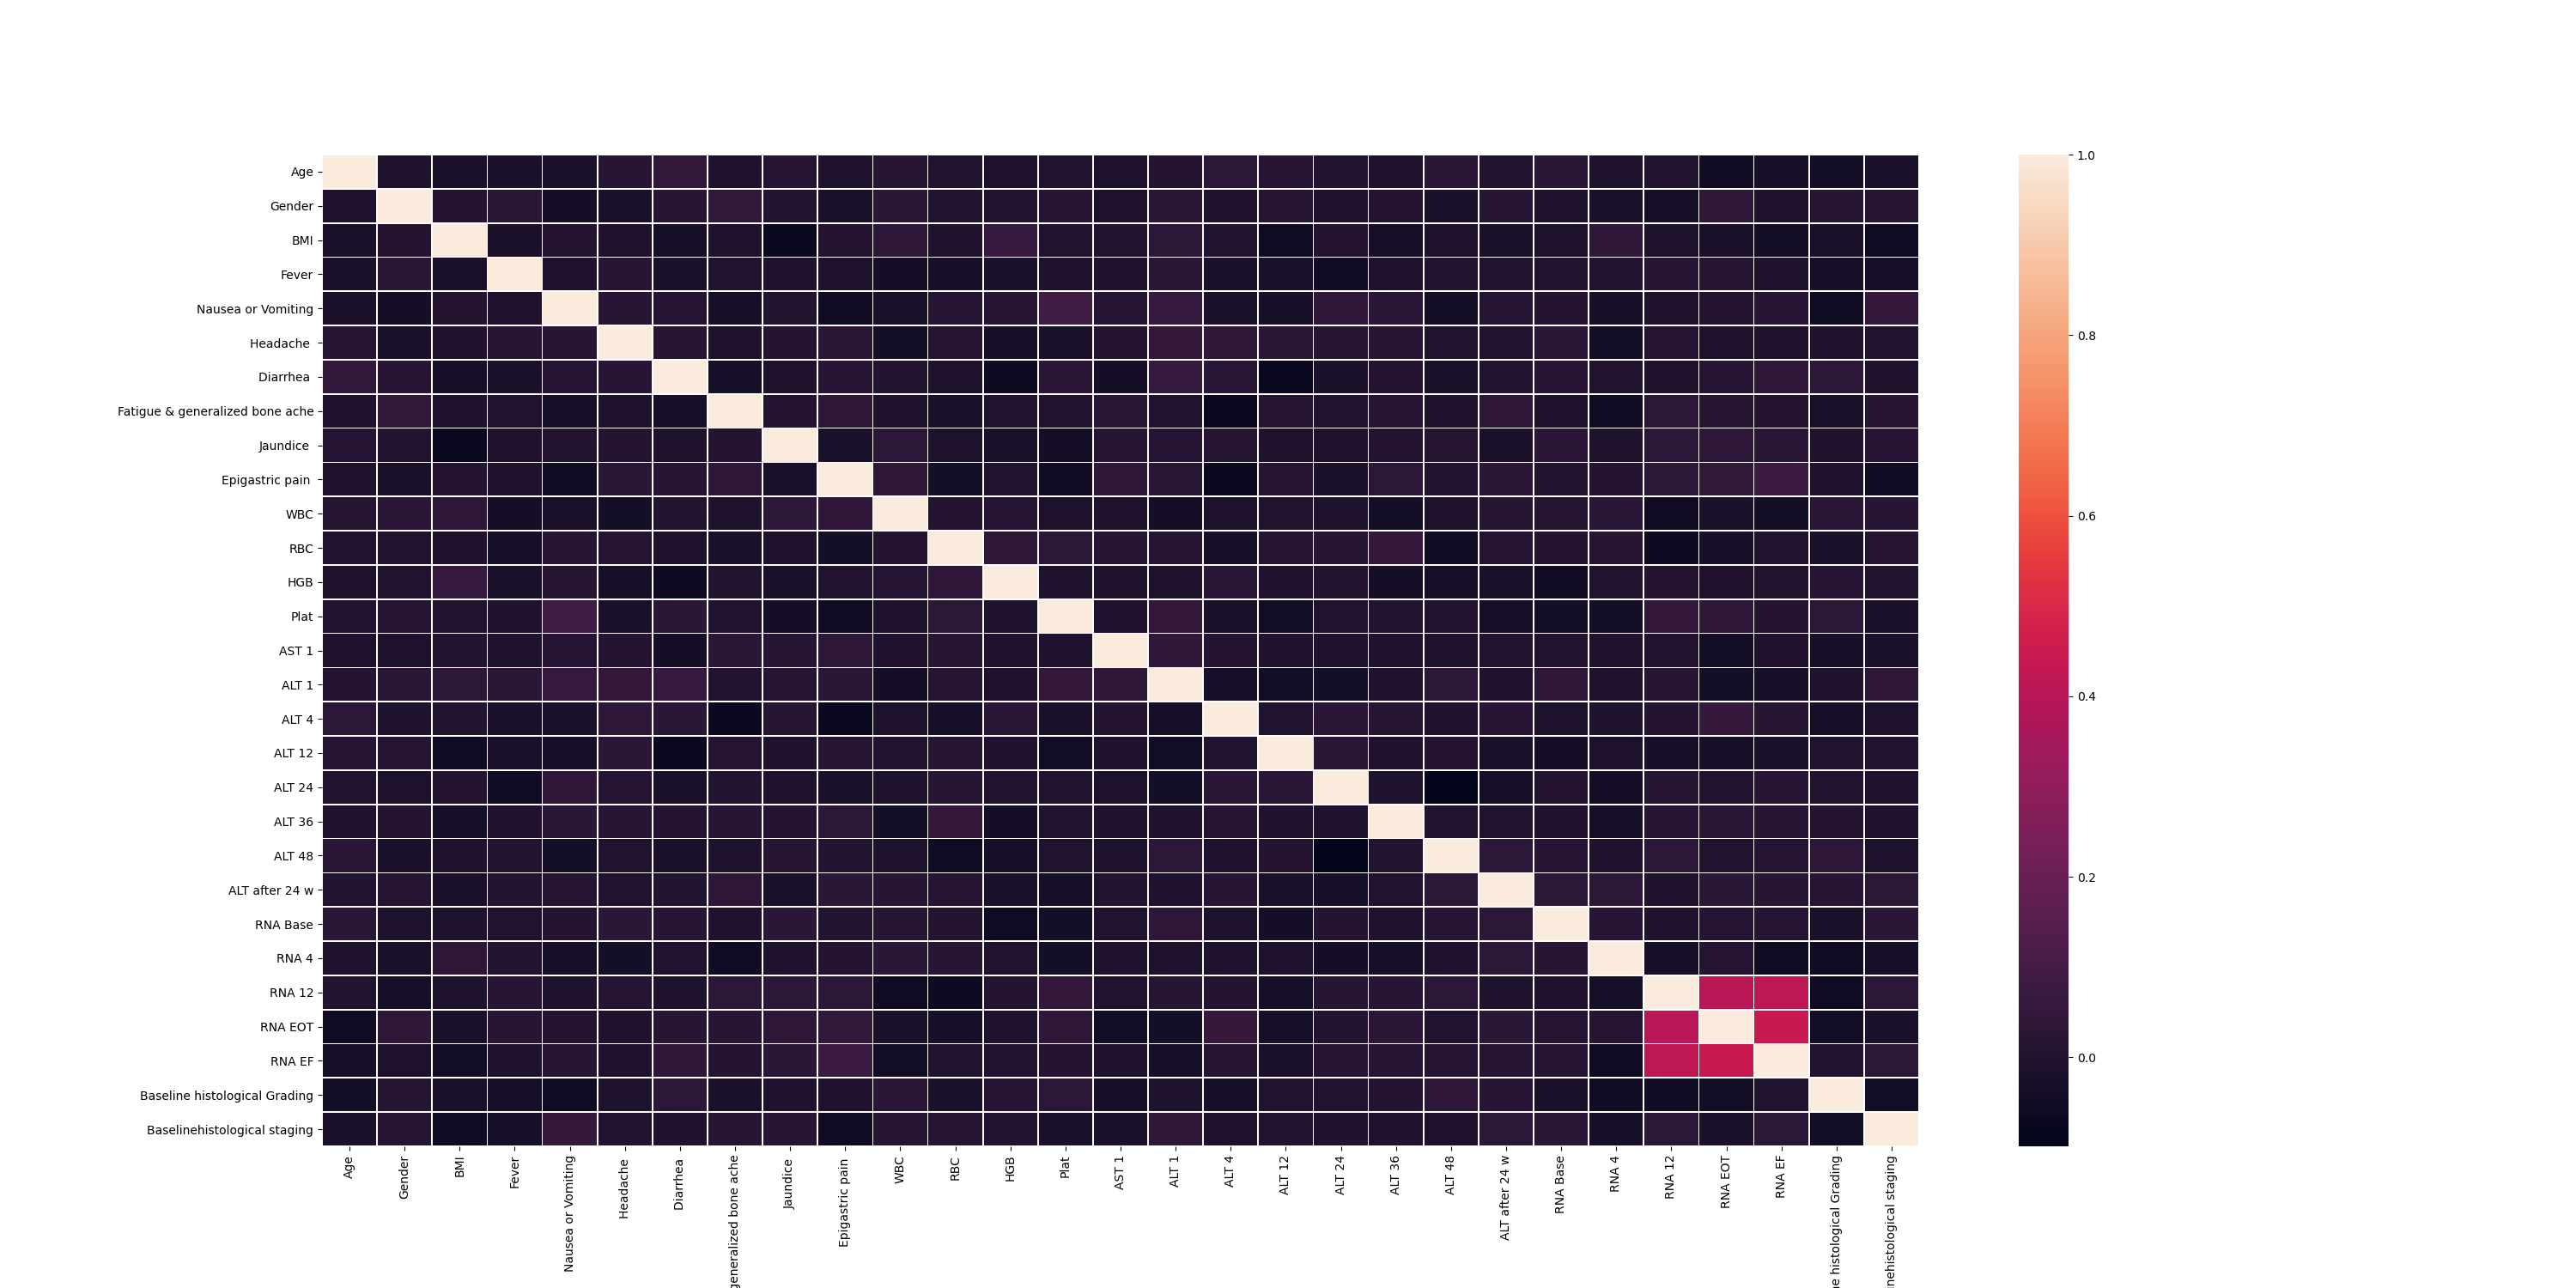
\includegraphics[width=1\columnwidth]{figures/matrx_corr.png}
    \caption{Matrice di Correlazione}
    \label{fig:matr_corr}
\end{figure}

\subsection{Clustering per valutazione della complessità del problema}

Ho voluto trattare inizialmente i dati, anche quelli non discretizzati, per avere un'idea della difficoltà di classificazione del dataset. Per questa ragione è stato usato un algoritmo di clustering su 3 features, sia discretizzate che non, (Baseline histological Grading, RNA EOT, RNA EF), che, in accordo con i medici, potrebbero ben "classificare" le 4 famiglie di fibrosi. La scelta di un numero così basso di features (3 su 28) è stato effettuato per rappresentare graficamente i dati con un numero notevolmente inferiore di features. 

Prima di tutto però, partiamo col definire cos'è il clustering. Il clustering appartiene alla famiglia degli algoritmi non supervisionati e consiste nell'etichettare una mole di dati senza conoscere l'etichette, scoprendo raggruppamenti tra dati simili tra loro. Questa tipologia di algoritmi è utilizzata sopratutto quando, come in molti dei casi reali, non si possiedono etichette e non si ha la potenza computazionale e/o il tempo per etichettare tutti i dati. Infatti i punti "simili" tra loro finiscono nello stesso gruppo, mentre quelli diversi finiscono in gruppi diversi. Per raggruppare i punti si devono considerare principalmente 2 aspetti:
\begin{itemize}
    \item Il primo è quello di misurare la distanza tra questi punti, che può essere euclidea, di Manhattan, di Mahalanobis. Ogni definizione diversa di distanza può creare cluster di diversa forma.
    \item Il secondo è quello di valutare la qualità di un clustering attraverso, per esempio, la distanza tra i baricentri di ogni cluster
\end{itemize}
I dati in questione da me utilizzati per il clustering non sono stati normalizzati o standardizzati poichè questo potrebbe influire negativamente sulla bontà del clustering e ho voluto appositamente utilizzare i dati "crudi" del dataset per evidenziare eventuali pattern nascosti. 
L'algoritmo da me utilizzato è il K-Means che cerca di minimizzare una certa funzione obbiettivo.
Prima di tutto però bisogna rappresentare un insieme di N punti attraverso un solo punto x*. Per farlo si può utilizzare il criterio della minima distanza euclidea:

\begin{equation}
    J(\mathbf{x*})=\sum_{N}^{n=1}\left \| \mathbf{x_{n}-x*}  \right \|^{2}
\end{equation}

Il minimo di questa funzione è il punto medio dei dati, ovvero il baricentro. Ecco quindi che si possono raggruppare N punti in k cluster considerando come funzione l'errore quadratico totale considerando i cluster come gli insiemi C1, C2,...,Ck e come centri i rispettivi baricentri. 
L'algoritmo in esame è il K-Means che approssima il minimo di \begin{math}J_e\end{math} definita come:

\begin{equation}
    J_{e}=\sum_{k}^{q=1}\sum_{x\epsilon C_{q}}^{}\left \| x-c_{q} \right \|^{2}
\end{equation}

Il numero di cluster scelto, k, è un iperparametro e questo sta a significare che dobbiamo sceglierlo con un buon criterio. Il metodo per trovarlo in modo oppurtuno è rappresentare il rapporto di \begin{math}J_k/J_1\end{math}, chiamata inertia, in funzione di k. Quello che è stato fatto è riportare graficamente questa funzione, monotona descrescente, in modo tale da poter osservare nel "gomito" della funzione il valore ottimo di k. Sono stati presi in analisi sia i valori discretizzati che non discretizzati. Si può notare come il valore ottimo k con i valori non discretizzati sia molto maggiore di 4 (ovvero il numero di classi del nostro problema) e, anche se c'è un visibile miglioramento coi dati discretizzati, rimane comunque molto alto. Questo risultato ci induce a pensare che il problema sia molto difficile da classificare attraverso sole 4 classi (fig.\ref{fig:k_means1}). 
Come si puo notare dalla fig.\ref{fig:k_means2} il clustering, con k=4, avviene con successo, clasterizzando le 4 classi della target in modo abbastanza netto. Ciò significa che queste 3 features sono molto rilevanti per determinare la gravità della fibrosi di un paziente, anche se con la discretizzazione diventa meno evidente.

\begin{figure}[H]
    \centering
    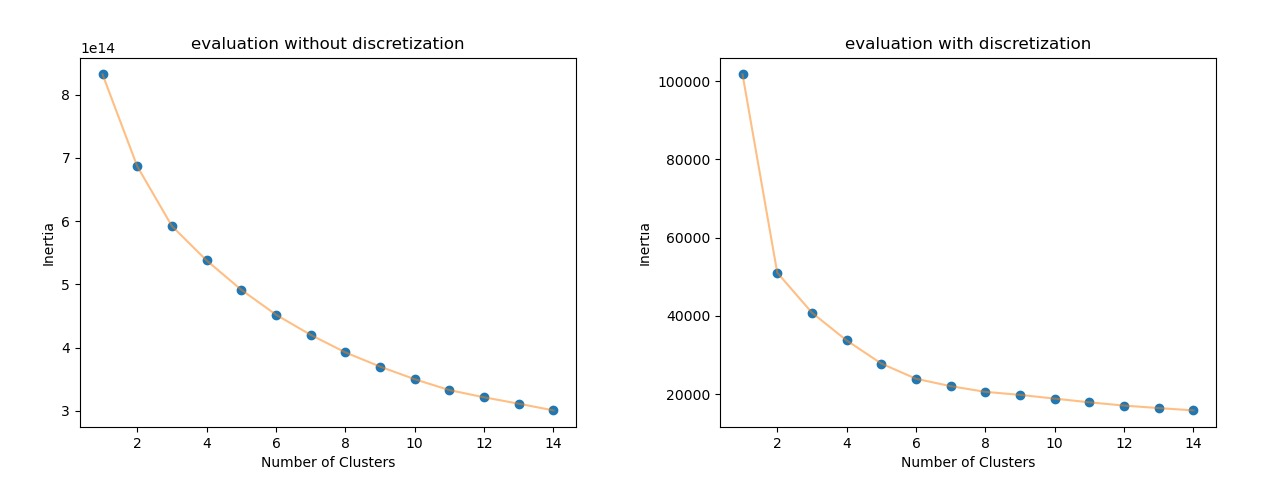
\includegraphics[width=1\columnwidth]{figures/Kmeans_K.jpg}
    \caption{K means, variazione del numero di k cluster}
    \label{fig:k_means1}
\end{figure}
\begin{figure}[H]
    \centering
    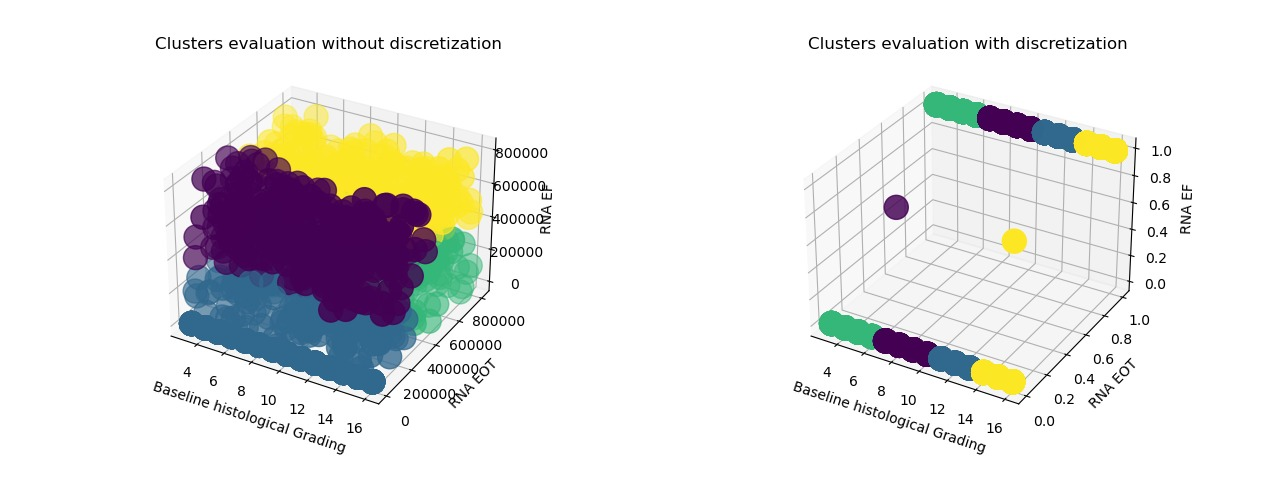
\includegraphics[width=1\columnwidth]{figures/clusters.jpg}
    \caption{Plot 3D del clustering con 3 features}
    \label{fig:k_means2}
\end{figure}

\subsection{Criterio di Splitting del dataset}

Ho voluto riservare al Training set, ovvero la porzione di dati su cui i modelli si addestreranno, un 80\% mentre per il Test set per la valutazione dei risultati un 20\%. Quindi 1.108 su 1385 samples sono riservati al training e 277 per il test.

\begin{figure}[H]
    \centering
    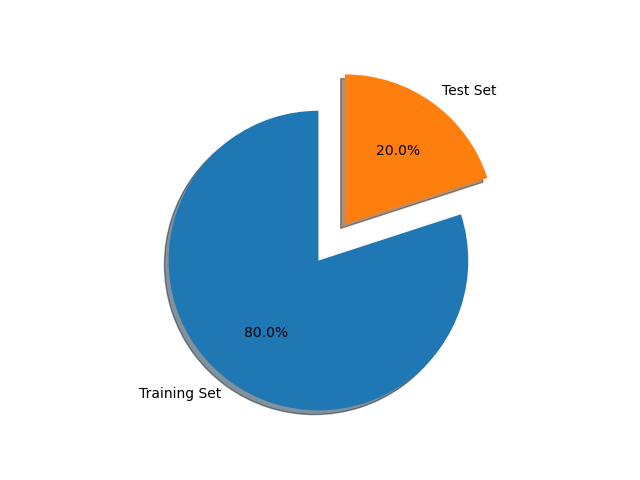
\includegraphics[width=0.75\columnwidth]{figures/pieSplitting.png}
    \caption{Splitting}
    \label{fig:splitting}
\end{figure}

    





\section{Discussione dei Modelli}\cite{STATISTICALLEARNING}

In questa sezione si discuteranno quali motivi mi hanno spinto a scegliere i modelli utilizzati e come essi funzionano.
\subsection{Scelta dei Modelli}

Ho voluto scegliere algoritmi di classificazione poichè, riferendomi all'EDA (subsection. \ref{ssec:EDA}), in particolare alla matrice di correlazione, fig.\ref{fig:matr_corr}, non vi è nessuna feature correlata all'uscita in modo lineare e quindi non ho potuto applicare nessun modello di regressione lineare. Inoltre le uscite sono valori discreti, quindi perfetti per una classificazione.
Per la mia classificazione ho voluto utilizzare due modelli:
\begin{itemize}
    \item K-Nearest Neighbors
    \item Decision Tree
\end{itemize}
La scelta del primo è dovuta al fatto che è un algoritmo semplice e, sebbene all'aumentare dei dati il KNN sia decisamente lento per le ragioni sotto riportate, per la mia mole di dati è abbastanza veloce. Non c'è inoltre bisogno di costruire un vero e proprio modello come nel caso di altri algoritmi.
\break La scelta del secondo modello, il Decision Tree, è dovuto al fatto che è molto veloce nel classificare nuovi dati. Per giunta, la visualizzazione dell'albero decisionale è di facile comprensione sopratutto in ambito medico. Quindi un dottore potrebbe facilemente interpretare il modello e classificare il tipo di fibrosi di un nuovo paziente. 

\subsection{K-Nearest Neighbor}

Il principio del KNN è diverso dagli altri algoritmi di apprendimento. Infatti esso non scarta il training set una volta che il modello è costruito, mantenendo tutto il training set in memoria. L'algoritmo, una volta che vede un nuovo sample x, trova i "k" training samples più vicini a x e ritorna la label maggioritaria tra questi samples, ovvero per i casi di regressione la media, per i casi di classificazione la moda. La vicinanza di due samples è data da una funzione di distanza. Essa può essere di diversi tipi, come per esempio:
\begin{itemize}
    \item Distanza Euclidea
    \item Distanza di Chebychev
    \item Distanza di Mahanattan
\end{itemize}
La distanza euclidea, con \begin{math}q\end{math} indicante un punto in molteplici dimensioni, può essere definita come:
\begin{equation}
    d(q^{i},q^{l})=\sqrt{\sum_{j=1}^{p}(q_{j}^{(i)}-q_{j}^{(l)})^{2}}
\end{equation}
Il numero k di vicini è un iperparametro e per questo dev'essere "settato" correttamente, altrimenti con k molto piccoli o troppo grandi si potrebbe avere una predizione molto instabile. Se k aumenta, si diminuisce il rumore che compromette la giusta classificazione, tuttavia se k diminuisce la classificazione non è facilmente determinabile.  

\begin{figure}[H]
    \centering
    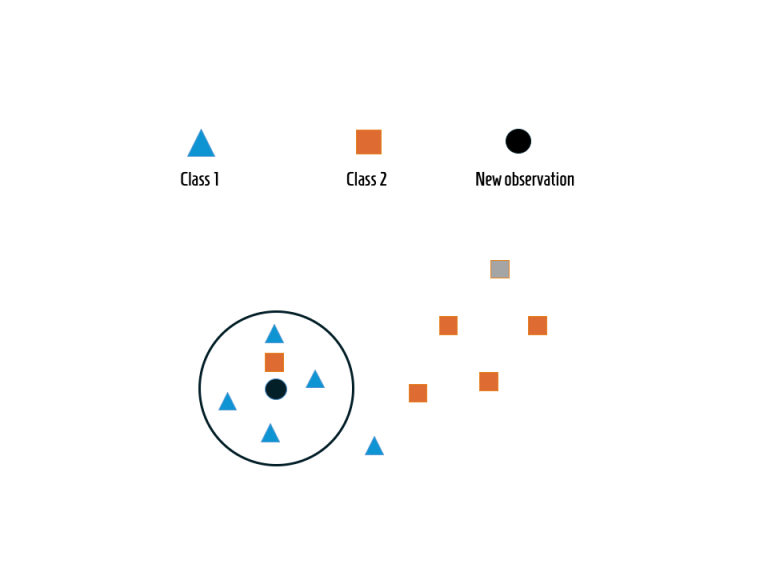
\includegraphics[width=0.65\columnwidth]{figures/k-nearest-neighbor-768x576.png}
    \caption{KNN}
    \label{fig:target}
\end{figure}

\subsection{Decision Tree}

Il Decision tree o albero decisionale è un algoritmo appartenente alla famiglia dei modelli supervisionati. Esistono due tipo di Alberi, quelli per la classificazione e quelli per la regressione. Il discriminante è che il primo utilizza dati discreti come nel mio caso, il secondo valori continui.
Un albero è costuituito da 3 elementi cardine:
\begin{itemize}
    \item Nodi: testano il valore di un certo attributo
    \item Foglie: Sono i nodi terminali, che predicono il risultato
    \item Rami: sono i collegamaneti tra i risultati dei test e il nodo successivo, o foglia
\end{itemize}
I dati sono continuamente suddivisi in base ad un certo parametro. Infatti in questo grafo aciclico (l'albero) uno specifico vettore feature viene esaminato e, se il valore della feature è sotto una certa soglia, viene seguito il ramo di sinistra, altrimenti quello di destra. Questo algoritmo, come fa supporre il nome, impara attraverso i dati che ha a disposizione.
\newline Vengono seguite le seguenti regole:
\begin{itemize}
    \item Seleziona un test per il nodo radice e crea un branch per ogni possibile risultato di questo test
    \item Divide le istanze in sottoinsiemi, uno per ogni ramo che si estende dal nodo
    \item Ripete in modo ricorsivo, usando solo istanze cha raggiungono il ramo
    \item Ferma la ricorsione per un ramo se tutte le sue instanze hanno lo stesso output
\end{itemize}
Quello che si cerca di effetture, per evitare di considerare ogni possibile partizione dello spazio delle features, è usare il \textbf{recursive binary splitting}, ovvero selezionare il cutpoint e le features che portano alla maggiore impurità dei nodi. Un nodo è definito \textbf{puro} quando tutti i samples nello stesso "split" hanno lo stesso valore di uscita. Come misurare l'impurità di un nodo? Attraverso l'indice di Gini, cioè un valore tra 0 e 1 in cui il valore 0 indica che tutti gli elementi appartengono ad una specifica classe mentre 1 evidenzia che gli elementi sono distribuiti in modo totalmente casuale in varie classi. Dunque un indice di Gini che vale 0.5 suggerisce che gli elementi sono equamente distribuiti nelle varie classi.
\newline Purtroppo però i Decision Tree sono soggetti all'overfitting, ovvero si adatta fortemente ad uno specifico training set e questo comporta a predire valori mai visti in modo completamente anomalo. Inoltre minimi cambiamenti dei dati di training possono comportare una logica di decisione completamente diversa.
\begin{figure}[H]
    \centering
    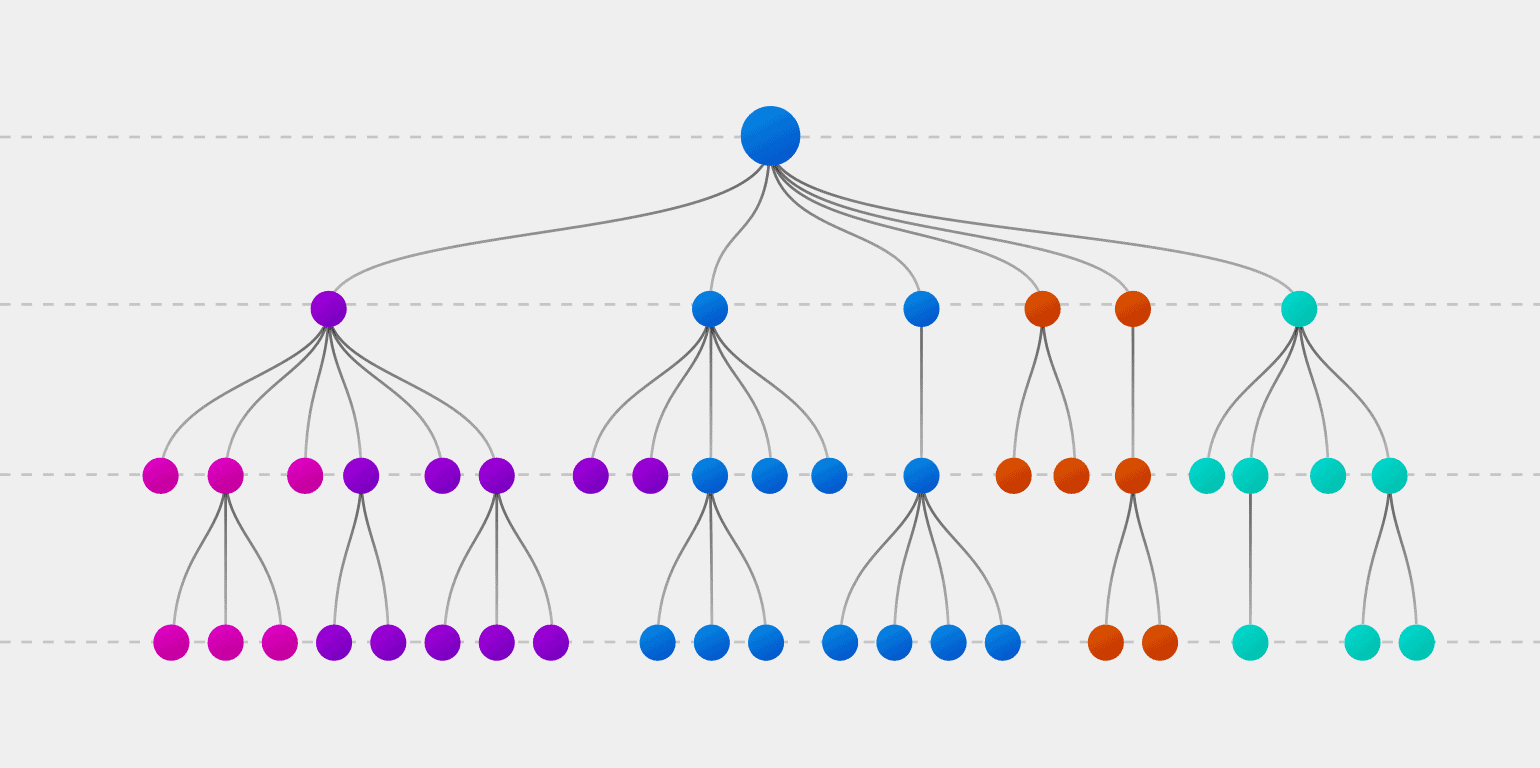
\includegraphics[width=0.65\columnwidth]{figures/Decision-Trees.png}
    \caption{Albero decisionale}
    \label{fig:target}
\end{figure}

\section{Dettagli Implementativi}\cite{STATISTICALLEARNING}\cite{ML2}\cite{StackOverflow}
In questa sezione si discuteranno le scelte di implementazione come preprocessing, scelta degli iperparametri, descrizione dei criteri di valutazione.

%preprocessing
\subsection{Preprocessing}

La strategia di preprocessing dei dati è essenziale nel caso in cui si abbiano features non rilevanti per l'output, troppe features rispetto al numero di samples, range di valori del dataset estremamente grandi, quantità di samples troppo grande per essere computata in tempi ragionevoli. 
\newline Prima di effetture il vero preprocessing, ho creato delle funzioni che mi permettessero di cambiare i valori dei dati nei range consigliati dai medici. Per questo motivo ho usato delle mie funzioni "custom" per poter discretizzare i dati entro i range prescelti dai medici.
\newline Per quanto riguarda il target non ho effettuato nessun tipo di operazione in quanto era già convertito in 4 valori numerici.
\newline Le strategie più utilizzate, quando si hanno valori compresi tra range molto ampli, sono quelle di standardizzazione e normalizzazione dei dati.
Standardizzare i dati vuole dire portare i valori di una variabile aleatoria X con varianza \begin{math}\sigma\end{math} e media \begin{math}\mu\end{math} ad una variabile Z, con distribuzione standard, ovvero media zero e varianza uno:
\begin{equation}
    Z=\frac{X-\mu}{\sigma}
\end{equation}
Questo procedimento è utilizzato per riportare alcuni valori molto grandi di features diverse nelle stesso range. Così facendo non ci saranno valori con un peso maggiore rispetto ad un altro.
La normalizzazione segue lo stesso concetto, tuttavia la formula che la descrive è diversa e la nuova variabile "vivrà" in un range tra 0 e 1:
\begin{equation}
    Z=\frac{X-min}{max-min}
\end{equation}
dove \textit{min e max} sono rispettivamente il minimo e il massimo valore del dominio dove vivono i valori della feature stessa.
\newline Per la mia tiplogia di problema, non ho voluto appositamente usare questi due metodi di preprocessing poichè non l'ho ritenuto necessario. Nessuno dei valori delle feature, essendo discretizzati precedentemente, necessita di essere standardizzato o normalizzato nè ci sono valori molto grandi. Per di più ci sono valori discreti di molte features, che assumono valore o 0 o 1: applicando questi metodi i loro valori sarebbero stati gli stessi, sprecando solamente delle risorse computazionali. 


Per quanto concerne il mio datset ho voluto utilizzare due strategie:
\begin{itemize}
    \item Rimozione delle features non utili alla classificazione sulla base dell'EDA
    \item Usare il metodo di selezione di k features con K-Best
\end{itemize}

\newline Come rilevato precedentemente (vedi fig. \ref{fig:distr_features_1}) nel dataset è presente una feature con sempre lo stesso valore, ovvero RNA base. Per questa ragione ho eliminato questa feature. Si è passati quindi da 28 features a 27 features. Questo tipo di operazione di features selection è stata effettuata "manualmente" osservando i risultati dell'EDA. Questi tipi di features selection basati sull'EDA sono noti come \textbf{filter methods}. Ho deciso di mantere anche le altre features con bassa varianza poichè questi valori potrebbero essere necessari ai fini della classificazione essendo valori estratti da referti medici. Inoltre testando i modelli ed eliminando queste features, le perfomance dell'algoritmo calavano notevolmente, in particolare l'accuracy. Così ho deciso di seguire un'altra strada per un'ulteriore features selection senza però applicarlo manualmente. Questa operazione è stata effettuata scartando la colonna corrispondente alla feature "RNA Base" che tramite la funzione di VarianceThreshold con parametro di input di default "threshold"=0. Ciò sta ad indicare che questa funzione eliminerà le features con varianza nulla come appunto RNA Base. 
\newline Non avendo forti correlazioni tra le features e l'output target ho proceduto come segue.
\newline Mi sono preoccupato di selezionare le k features più rilevanti, usando un metodo di preprocessing chiamato "K-Best". Questo metodo seleziona le k migliori features basandosi sulla varianza delle features e quanto queste influiscono sull'uscita. Per determinare quale sia il valore ottimale di k, ho testato un range tra 12 e 27 (di k). Il test è stato effettuato per ognuno dei 2 algoritmi selezionati per la classificazione (KNN e Decision Tree ), riportando il k che migliora l'accuracy. Da ciò è emerso che il valore k ottimale per K-nearest neighbors è 24 mentre, per il Decision Tree è 19, vedi fig.\ref{fig:features_selectionKNN}
\newline Il funzionamento di KBest è semplice: prendere in input il training set e "fittarlo" in base all'output riferito allo stesso train set e selezionare le k features per le quali si ha uno "score" elevato. Questo score può essere misurato attraverso diversi test, tra i quali \begin{math}\textbf{\chi^{2}}\end{math} da me utilizzato. Questo test misura la dipendenza tra una variabile (in questo caso la feature) e la variabile target, escludendo le features che sono più indipendenti dall'output e quindi inutili per la classificazione. 
Selezionare meno features comporta uno sforzo computazionale drasticamente minore per gli algoritmi di Machine Learning, con lo svantaggio di sacrificare alcuni dati. 
Riporto in una tabella le features selezionate per ogni algoritmo, tab. \ref{tab:features_selected}

\begin{table}[ht]
\centering
\begin{tabular}{@{}lcc@{}}
\toprule
   & \multicolumn{1}{l}{\textbf{Number of features selected}} & \textbf{Features selected}                                                                                                                                                                                                                                                                                                                                                                              \\ \midrule
\multicolumn{1}{|l|}{\textit{For KNN}}           & \multicolumn{1}{c|}{24}                                  & \multicolumn{1}{c|}{\begin{tabular}[c]{@{}c@{}}'Age', 'Gender', 'BMI', 'Fever',\\  'Nausea or Vomiting', 'Headache ', 'Diarrhea '\\  'Fatigue \& generalized bone ache' 'Jaundice ',\\  'Epigastric pain ', 'WBC',\\  'RBC', 'HGB', 'Plat', 'AST 1',\\  'ALT 12', 'ALT 24', 'ALT 36', 'ALT 48',\\  'ALT after 24 w', 'RNA 12',\\  'RNA EOT', 'RNA EF',\\  'Baseline histological Grading'\end{tabular}} \\ \midrule
\multicolumn{1}{|l|}{\textit{For Decision Tree}} & \multicolumn{1}{c|}{19}                                  & \multicolumn{1}{c|}{\begin{tabular}[c]{@{}c@{}}'Age', 'Gender', 'BMI' 'Fever',\\  'Nausea or Vomiting', 'Headache ', 'Diarrhea '\\  'Fatigue \& generalized bone ache', 'Jaundice ',\\  'Epigastric pain ', 'WBC',\\  'HGB', 'Plat' ,'ALT 36' ,'ALT after 24 w',\\ 'RNA 12', 'RNA EOT', 'RNA EF',\\  'Baseline histological Grading'\end{tabular}}                                                      \\ \bottomrule
\end{tabular}
\caption{ Le features selezionate per i due algoritmi attraverso KBest}
\label{tab:features_selected}
\end{table}
\begin{figure}[H]
    \centering
    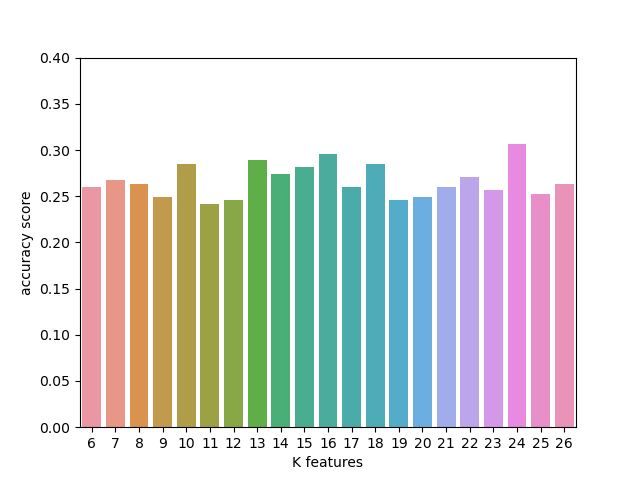
\includegraphics[width=0.5\columnwidth]{figures/KBEST_KNN.png}
    \caption{Accuracy al variare di K in KNN, con K: numero di features}
    \label{fig:features_selectionKNN}
\end{figure}

\begin{figure}[H]
    \centering
    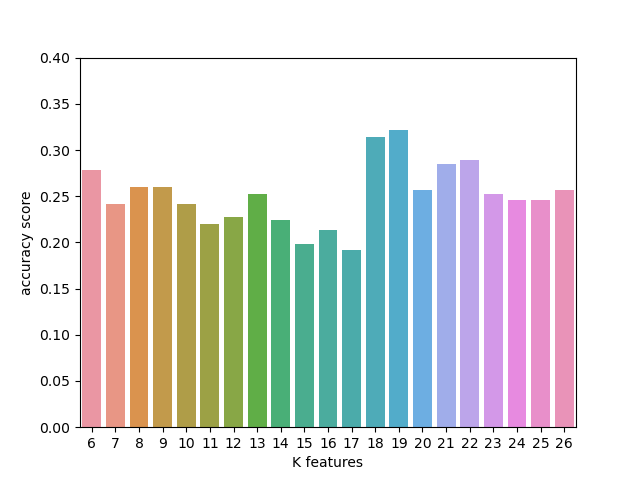
\includegraphics[width=0.5\columnwidth]{figures/KBestDT.png}
    \caption{Accuracy al variare di K in Decision Tree, con K: numero di features}
    \label{fig:features_selection_DT}
\end{figure}




\subsection{Varianti dei Modelli}

Come discusso, i modelli utilizzati per la classificazione sono Decision Tree e KNN.
\newline Questi "modelli" sono stati implementati sia con il preprocessing che senza preprocessing. Infatti, il primo è stato addestrato dopo avere effettuato la feature selection. Il secondo invece è stato addestrato con tutte le 29 features. Inoltre, per ognuna di queste due versioni sono state implementate le varianti con e senza cross validation, così da poter valutare quale performasse di più. In tutto quindi ci sono 6 modelli. Inoltre sono stati presi in esame i due migliori modelli, con accuracy più alta, e sono stati messi in ensamble come viene discusso in \ref{ssec:Ensemble}.



\subsection{Cross validation}

Prima di introdurre la Cross Validation, o convalida incrociata, ci tengo a spiegare l'overfitting e l'underfitting.
\newline L'overfitting avviene quando il modello si trova in una condizione di sovradattamento, ovvero quando esso diventa troppo complesso e specifico per i dati di training che sta processando. Questo sovradattamento alle caratteristiche dei dati del training, porta il modello a non prevedere nuovi dati, avendo dunque risultati performanti in caso di training e risultati scarsi in caso di test. Si parla dunque di alta varianza, ovvero si presta troppa attenzione sui dati di training.
\newline L'underfitting invece avviene quando il modello non riesce ad approssimare bene i dati di training e quindi risulta inadatto anche ai dati di test. In questo caso si parla di alto bias e modello troppo semplice. 
\newline Per trovare il giusto compromesso, si effettua quella che viene chiamata \textbf{cross validation}. Questa tecnica ci permette di scegliere gli iperparametri ottimali del modello ("model selection").
Esistono diverse tecniche di cross validation, tra cui:
\begin{itemize}
    \item \textbf{Holdout}: Una porzione del training set viene splittata una tantum tra i dati di addestramento e quelli per valutarne le prestazioni, appunto, il validation set. Ciò però può determinare basse o alte prestazioni poichè dipende da quali samples sono finiti nel training e nel validation set
    \item \textbf{K-Fold}: Il training set viene diviso in k parti, dette fold, in cui k-1 vengono usate come trining e la restante come validation. Iterando k volte, cambiando ad ogni step quale porzione venga utilizzata come validation set, si ottengono delle prestazioni con cui si effettua la media sui k run.
    \item \textbf{Leave-One-Out}: il training set viene diviso in n-1 samples, il validation con solo un sample. Ripetendo n volte, si ottiene lo scoring come media delle n prestazioni sugli n run.
\end{itemize}
Esiste poi la "Stratificazione", ovvero si fa in modo (che si usi KFold o Holdout) di avere \textbf{proporzionalmente} il numero di sample di ciascuna classe nei fold (in Kfold) e nel training e nel validation set (nella Holdout).
La tecnica da me utilizzata è stata KFold con startificazione. Infatti ho utilizzato la funzione di sklearn GridsearchCV settando i seguenti valori: (di default) "cv": 5 (ovvero sfrutta 5 fold con Kfold), "estimator": modello (KNN o Decision Tree), "param\_grid": parametri selezionati e scoring: "accuracy" (ovvero tiene conto per le performance l'accuracy come parametro di ricerca della selezione degli iperparmetri. Viene discusso in seguito perchè ho scelto proprio l'accuracy come metrica).
Internamente e di default questa funzione utilizza la stratificazione, per cui non ho dovuto specificare nulla nè creare funzioni custom per implementarla.
\newline Gli iperpametri presi in causa sono stati per il KNN:
\begin{itemize}
    \item "n\_neighbors": come già visto prima, il numero di vicini
    \item "weights": ovvero i pesi. Può essere sia "uniform", ovvero ogni punto del "vicinato" ha lo stesso peso, che "distance", ovvero il peso dei vicini dipende dall'inverso della distanza. Un vicino molto lontano pesarà meno di uno davvero prossimo al punto preso in esame.
    \item "p": che può assumere i valori "1" o "2". Il primo utilizza la distanza euclidea, il secondo quella di Mahnattan.
\label{parameters}
\end{itemize}
\newline Per il decision tree invece, sono stati presi in considerazione i seguenti iperparametri:
\begin{itemize}
    \item "max\_depth": la profondità dell'albero
    \item "criterion": misura della qualità dello split. Può essere di Gini o in base all'entropia. 
    \item "splitter": strategia per splittare un nodo. Può essere "best" per scegliere il migliore split o "random" per uno split casuale
\end{itemize}


\begin{table}[ht]
\centering
\begin{tabular}{@{}l|c|r|@{}}
\cmidrule(l){2-3}
                                            & \multicolumn{1}{l|}{\textbf{Iperparameters}} & \textbf{Range of values}  \\ \cmidrule(l){2-3} 
\multirow{3}{*}{\textit{For KNN}}           & n\_neighbnors                                & from 1 to 100, odd values \\ \cmidrule(l){2-3} 
                                            & weights                                      & uniform or distance       \\ \cmidrule(l){2-3} 
                                            & p                                            & 1 or 2                    \\ \cmidrule(l){2-3} 
\multirow{3}{*}{\textit{For Decision Tree}} & max\_depth                                   & from 1 to 100, odd values \\ \cmidrule(l){2-3} 
                                            & criterion                                    & Gini or Entropy           \\ \cmidrule(l){2-3} 
                                            & splitter                                     & best or random            \\ \cmidrule(l){2-3} 
\end{tabular}
\end{table}

\newline Dalla Cross Validation sono emersi i seguenti iperparametri ottimali:

\begin{table}[ht]
\centering
\begin{tabular}{@{}ll|c|r|@{}}
\cmidrule(l){3-4}
                                                                  &                                        & \multicolumn{1}{l|}{\textbf{Iperparameters}} & \textbf{Optimal value} \\ \midrule
\multicolumn{1}{|l|}{\multirow{3}{*}{\textit{For KNN}}}           & \multirow{3}{*}{With Preprocessing}    & n\_neighbnors                                & 67                     \\ \cmidrule(l){3-4} 
\multicolumn{1}{|l|}{}                                            &                                        & weights                                      & distance               \\ \cmidrule(l){3-4} 
\multicolumn{1}{|l|}{}                                            &                                        & p                                            & 1                      \\ \midrule
\multicolumn{1}{|l|}{\multirow{3}{*}{\textit{For Decision Tree}}} & \multirow{3}{*}{With Preprocessing}    & max\_depth                                   & 63                     \\ \cmidrule(l){3-4} 
\multicolumn{1}{|l|}{}                                            &                                        & criterion                                    & Entropy                \\ \cmidrule(l){3-4} 
\multicolumn{1}{|l|}{}                                            &                                        & splitter                                     & random                 \\ \midrule
\multicolumn{1}{|l|}{\multirow{3}{*}{\textit{For KNN}}}           & \multirow{3}{*}{Without Preprocessing} & n\_neighbnors                                & 95                     \\ \cmidrule(l){3-4} 
\multicolumn{1}{|l|}{}                                            &                                        & weights                                      & distance               \\ \cmidrule(l){3-4} 
\multicolumn{1}{|l|}{}                                            &                                        & p                                            & 1                      \\ \midrule
\multicolumn{1}{|l|}{\multirow{3}{*}{\textit{For Decision Tree}}} & \multirow{3}{*}{Without Preprocessing} & max\_depth                                   & 79                     \\ \cmidrule(l){3-4} 
\multicolumn{1}{|l|}{}                                            &                                        & criterion                                    & Entropy                \\ \cmidrule(l){3-4} 
\multicolumn{1}{|l|}{}                                            &                                        & splitter                                     & random                 \\ \bottomrule
\end{tabular}
\end{table}

\begin{figure}[H]
    \centering
    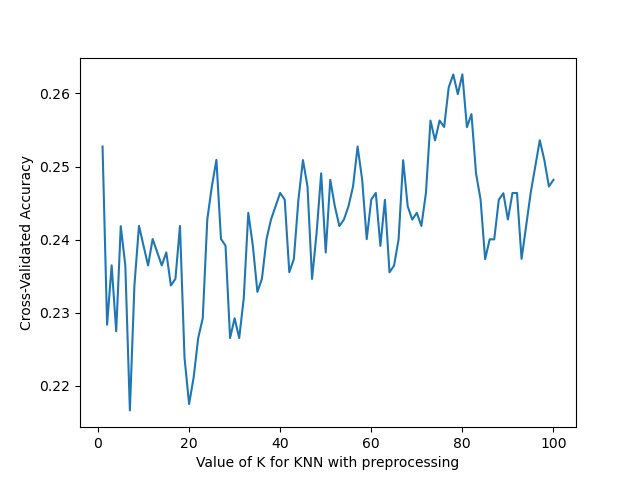
\includegraphics[width=0.55\columnwidth]{figures/K NeighBor Preproc.png}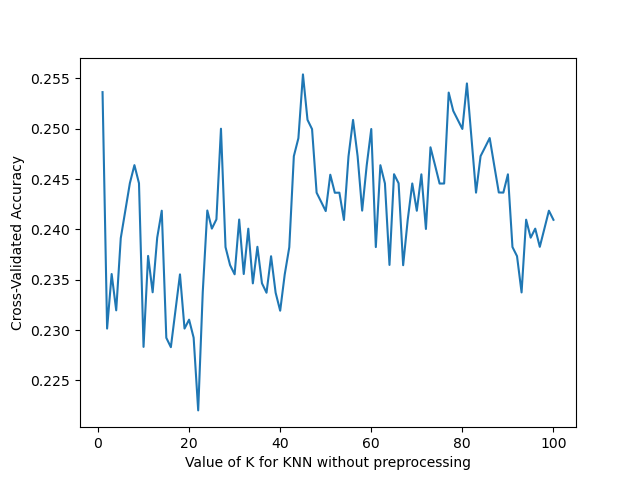
\includegraphics[width=0.55\columnwidth]{figures/K neight No Preproc.png}
    \caption{Cross Validation Accuracy al variare di K neighbor}
    \label{fig:target}
\end{figure}


\subsection{Ensemble}\label{ssec:Ensemble}

La tecnica di ensemble viene impiegata per combinare più modelli, detti \textbf{weak estimator}, per risolvere uno stesso problema. Vengono poi combinati per raggiungere un modello finale, \textbf{l'ensemble} per ottenere maggiori prestazioni. 
\newline Esistono diversi modi per effttuare l'ensemble, tra i quali:
\begin{itemize}
    \item \textbf{bagging}: si addestrano in parallelo n weak models e li si combina in ottica deterministica
    \item \textbf{boosting}: si addestrano in sequenza n modelli e li si concatena in maniera deterministica. Per cui ogni weak learner dipende dai precedenti.
    \item \textbf{stacking}: ogni modello viene considerato diverso (eterogeneità) e si addestra in parallelo in modo indipendente. Successivamente si combinano tutti i weak learner e si addestra il meta modello finale per effettuare predizioni sulla base dell'output designato dai weak learner.
\end{itemize}
L'ensemble, che è stato da me utilizzato, è tramite la tecnica di bagging, cioè un meta-stimatore di insieme che si adatta ai classificatori di base, ciascuno su sottoinsiemi casuali del set di dati originale e quindi aggrega le loro previsioni individuali (mediante voto o media) per formare una previsione finale. Ciò può inoltre ridurre la varianza dello stimatore base come il Decision Tree. Per questa ragione viene impiegato sui classificatori K-NearestNeighbor e Decision Tree che hanno più alto grado di accuracy.

\begin{figure}[H]
    \centering
    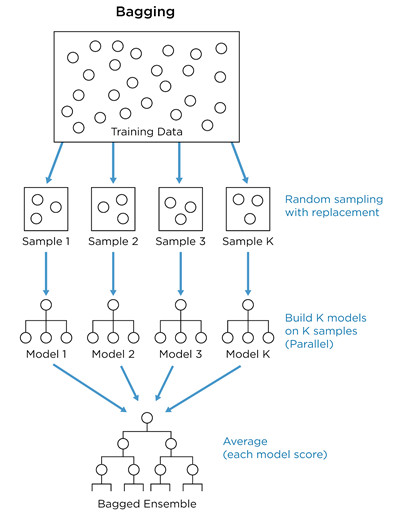
\includegraphics[width=0.35\columnwidth]{figures/Bagging_Ensemble.jpg}
    \caption{Bagging Ensemble}
    \label{fig:target}
\end{figure}

\subsection{Criteri di Valutazione}\label{ssec: Criteria}

I criteri per la valutazione e il confronto dei diversi algoritmi soono stati : 
\begin{itemize}\label{eq: confusion matrix}
    \item Accuracy: \begin{equation}
        Accuracy= \frac{TP+TN}{TP+TN+FP+FN}
    \end{equation}
    \item Precision: \begin{equation}
        Precision= \frac{TN}{TN+FP}
    \end{equation}
    \item Recall: \begin{equation}
        Recall= \frac{TP}{TP+FN}
    \end{equation}
    \item F1-score: \begin{equation}
        F1-score= \frac{2 *  Precision * Recall}{Precision + Recall}
    \end{equation}
    
\end{itemize}
Dove TP sono i \textit{True Positive}, TN sono i \textit{True Negative}, FP sono i \textit{False Positive} e i FN sono i \textit{False Negative}. 
\newline Avendo delle classi bilanciate nel daset, come mostrato nella fig. \ref{fig:target}, ho tenuto in considerazione l'accuracy come metrica di confronto più indicativa tra le prestazioni dei modelli. Da qui la scelta nella cross validation e nell'ensamble di usare come parametro "scoring" l'accuracy. Quest'ultima fornisce un'idea di quanti sample predetti sono effettivamente della classe giusta. L'accuracy "totale" sarebbe totalmente inappropriata nel caso di dataset sbilanciati, per i quali dev'essere valutata l'accuracy per \textbf{ogni} classe. Potrebbe infatti dare risultati fuorvianti, poichè avendo molte istanze della stessa classe, si avrebbe una accuracy molto alta proprio perchè l'algoritmo riesce a prevedere molto bene la classe che ha "visto" più volte, ma non riesce a discernere una classe da un'altra. In caso di sbilanciamento del dataset si tende a preferire l'F1-Score poichè, essendo una media armonica che unisce Precision e Recall in un unica metrica, attribuisce un peso maggiore ai valori piccoli. Quindi usare F1-Score è utile sopratutto nei casi in cui per una o più classi ci sono pochi positivi, come nei dataset sbilanciati. 
\newline I quattro valori \textsc{TP,TN, FP, FN} si possono visualizzare graficamente attraverso quella che viene definita come \emph{Confusion matrix}.

\begin{figure}[H]
    \centering
    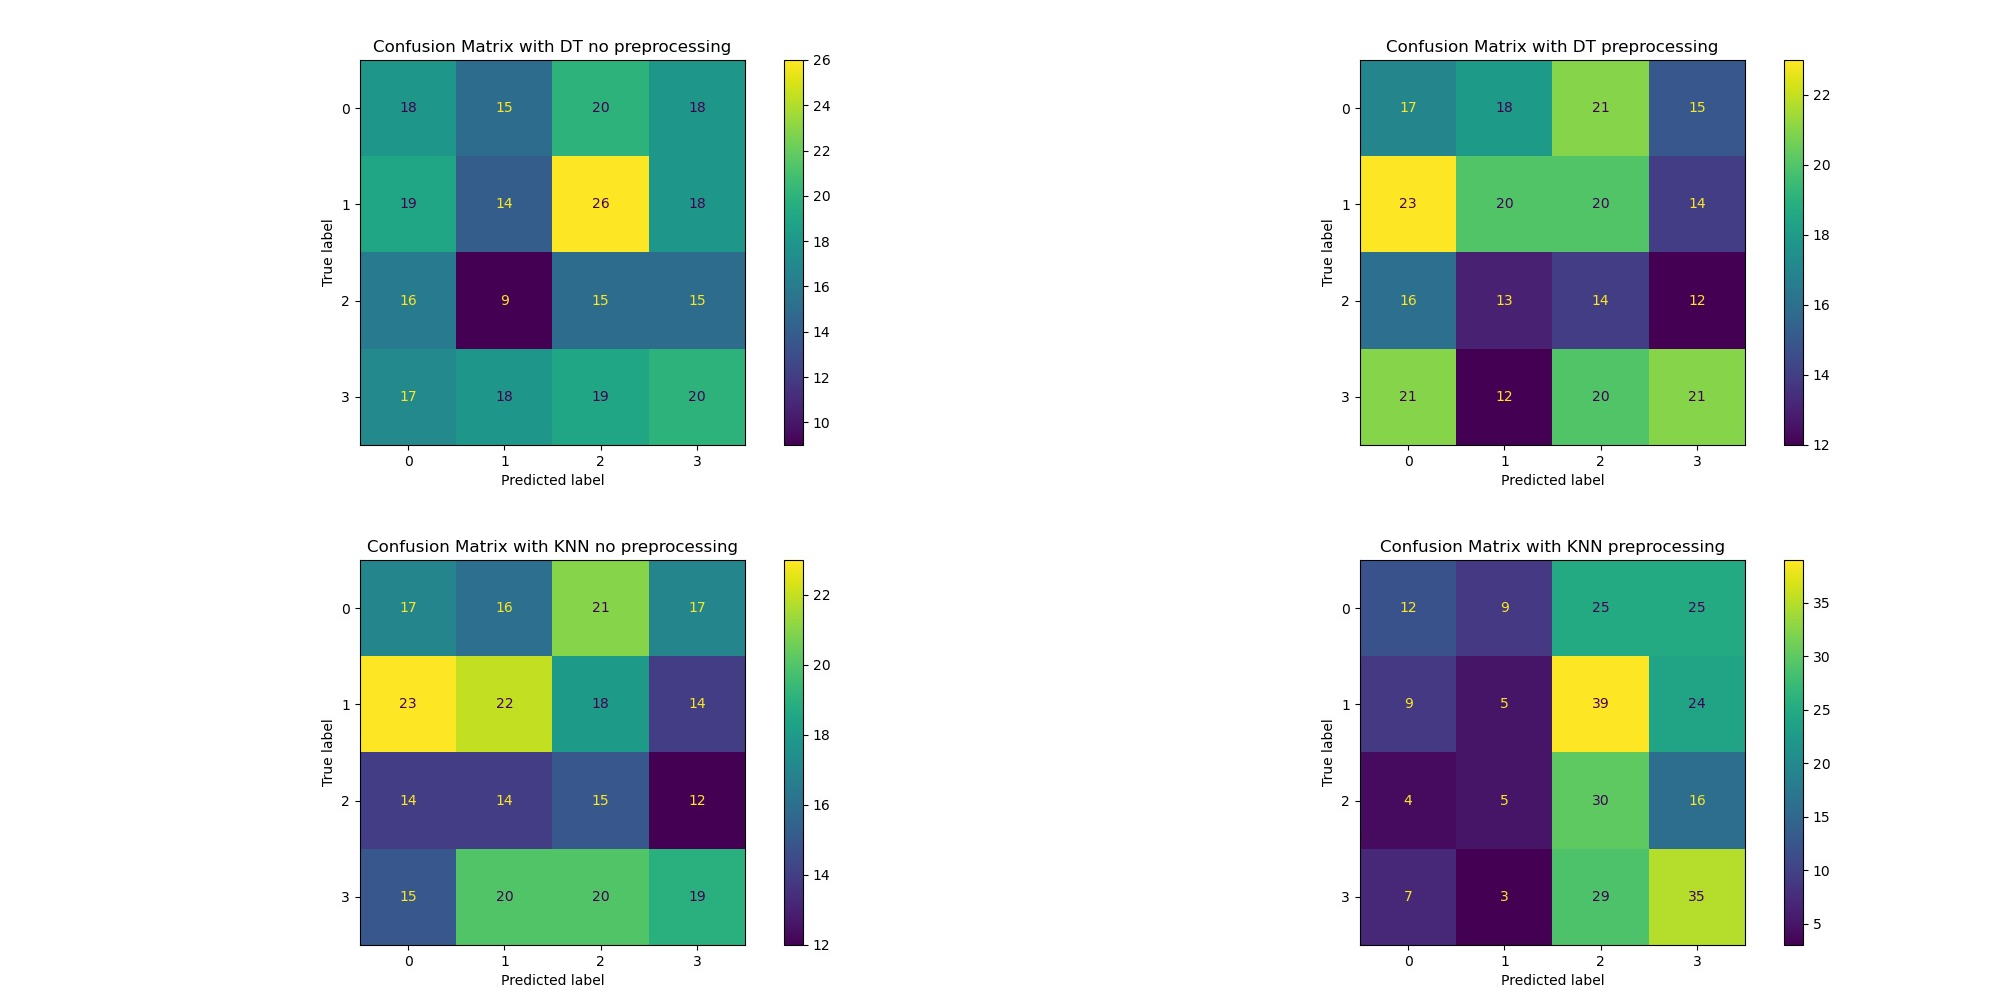
\includegraphics[width=1.1\columnwidth]{figures/Merge of Confusion Matrix.png}
    \caption{Le 4 confusion Matrix}
    \label{fig:target}
\end{figure}

Un'altra metrica importante da considerare è la ROC curve, ovvero la Relative Operating Characteristic. Infatti variando la soglia di classificazione si ottengono valori diversi per le metriche sopra menzionate. Per cambiamento della soglia di classificazione si intende la modifica dei paramentri del classificatore. 
La curva ROC viene creata tracciando il valore del True Positive Rate (TPR, frazione di veri positivi) rispetto al False Positive Rate (FPR, frazione di falsi positivi) a varie impostazioni di soglia. La curva ROC è quindi il tasso dei veri positivi in funzione del tasso dei falsi positivi.
\newline Per ultima abbiamo la curva Precision versus recall. Ricordo che la Precision o Specificity è la probabilità che un falso positivo ritornato dal classificatore sia corretto mentre la Recall è la percentuale di positivi riconosciuti correttamente. 


\section{Conclusioni e Risultati}
In questa sezione si confronteranno i risultati delle metriche menzionate nella sezione \ref{ssec: Criteria} e si faranno delle considerazioni finali.
\subsection{Analisi della Confusion Matrix}

Si può chiaramente notare come il modello K-NearestNeighbors con preprocessing predica discretamente bene le classi  "Many septa" e "Cyrrosis", ma faccia molta fatica a prevedere correttamente le prime due classi ovvero "Portal Fibrosis"  e "Few Septa". Mentre le altre varianti, Decision tree con preprocessing, senza preprocessing, e KNN senza preprocessing hanno una predizione molto scarsa su tutte e quattro le classi. (vedi fig. \ref{eq: confusion matrix}
\clearpage
\subsection{Performance per Modello}

Vengono riportate le metriche di prestazione di ciascun modello.

% Please add the following required packages to your document preamble:
% \usepackage{booktabs}
% \usepackage{multirow}
\begin{table}[ht]
\centering
\begin{tabular}{@{}lrcccc@{}}
\toprule
                                                                  & \multicolumn{1}{l}{}                                        & \multicolumn{4}{c}{\textbf{Average}}                                                                                                                                              \\ \midrule
\multicolumn{1}{|l|}{}                                            & \multicolumn{1}{l|}{}                                       & \multicolumn{1}{l|}{\textit{Precision}}    & \multicolumn{1}{r|}{\textit{Recall}}       & \multicolumn{1}{l|}{\textit{f1 score}}     & \multicolumn{1}{l|}{\textit{Accuracy}}     \\ \midrule
\multicolumn{1}{|l|}{\multirow{5}{*}{\textbf{For KNN}}}           & \multicolumn{1}{r|}{With Preprocessing}                     & \multicolumn{1}{c|}{0.30}                  & \multicolumn{1}{c|}{0.31}                  & \multicolumn{1}{c|}{0.27}                  & \multicolumn{1}{c|}{0.30}                  \\ \cmidrule(l){2-6} 
\multicolumn{1}{|l|}{}                                            & \multicolumn{1}{r|}{\multirow{3}{*}{Without Preprocessing}} & \multicolumn{1}{c|}{\multirow{3}{*}{0.27}} & \multicolumn{1}{c|}{\multirow{3}{*}{0.26}} & \multicolumn{1}{c|}{\multirow{3}{*}{0.26}} & \multicolumn{1}{c|}{\multirow{3}{*}{0.26}} \\
\multicolumn{1}{|l|}{}                                            & \multicolumn{1}{r|}{}                                       & \multicolumn{1}{c|}{}                      & \multicolumn{1}{c|}{}                      & \multicolumn{1}{c|}{}                      & \multicolumn{1}{c|}{}                      \\
\multicolumn{1}{|l|}{}                                            & \multicolumn{1}{r|}{}                                       & \multicolumn{1}{c|}{}                      & \multicolumn{1}{c|}{}                      & \multicolumn{1}{c|}{}                      & \multicolumn{1}{c|}{}                      \\ \cmidrule(l){2-6} 
\multicolumn{1}{|l|}{}                                            & \multicolumn{1}{r|}{Without Preprocessing, with CV}         & \multicolumn{1}{c|}{0.25}                  & \multicolumn{1}{c|}{0.25}                  & \multicolumn{1}{c|}{0.24}                  & \multicolumn{1}{c|}{0.25}                  \\ \midrule
                                                                  &                                                             &                                            &                                            &                                            &                                            \\ \midrule
\multicolumn{1}{|l|}{\multirow{5}{*}{\textbf{For Decision Tree}}} & \multicolumn{1}{r|}{With Preprocessing}                     & \multicolumn{1}{c|}{0.20}                  & \multicolumn{1}{c|}{0.26}                  & \multicolumn{1}{c|}{0.26}                  & \multicolumn{1}{c|}{0.26}                  \\ \cmidrule(l){2-6} 
\multicolumn{1}{|l|}{}                                            & \multicolumn{1}{r|}{\multirow{3}{*}{Without Preprocessing}} & \multicolumn{1}{c|}{\multirow{3}{*}{0.26}} & \multicolumn{1}{c|}{\multirow{3}{*}{0.26}} & \multicolumn{1}{c|}{\multirow{3}{*}{0.26}} & \multicolumn{1}{c|}{\multirow{3}{*}{0.26}} \\
\multicolumn{1}{|l|}{}                                            & \multicolumn{1}{r|}{}                                       & \multicolumn{1}{c|}{}                      & \multicolumn{1}{c|}{}                      & \multicolumn{1}{c|}{}                      & \multicolumn{1}{c|}{}                      \\
\multicolumn{1}{|l|}{}                                            & \multicolumn{1}{r|}{}                                       & \multicolumn{1}{c|}{}                      & \multicolumn{1}{c|}{}                      & \multicolumn{1}{c|}{}                      & \multicolumn{1}{c|}{}                      \\ \cmidrule(l){2-6} 
\multicolumn{1}{|l|}{}                                            & \multicolumn{1}{r|}{Without Preprocessing, with CV}         & \multicolumn{1}{c|}{0.25}                  & \multicolumn{1}{c|}{0.25}                  & \multicolumn{1}{c|}{0.24}                  & \multicolumn{1}{c|}{0.25}                  \\ \midrule
                                                                  & \multicolumn{1}{l}{}                                        &                                            & \multicolumn{1}{r}{}                       & \multicolumn{1}{l}{}                       & \multicolumn{1}{l}{}                       \\ \bottomrule
\end{tabular}

\caption{Performance e Confronto dei Modelli}
\label{tab:Performance_Modelli}
\end{table}
Si può notare chiaramente come il miglior classificatore sia il \textbf{KNN} con preprocessing e cross validation. 
L'accuracy migliore per il Decision Tree è quella utilizzando il preprocessing e cross validation. 
Il motivo per il quale si hanno metriche così basse è dovuto molto probabilemte alla complessità del problema trattato e il basso numero di samples del dataset (solo 1385). Sicuramente con un maggior numero di samples, quindi un numero maggiore di dati di nuovi pazienti soggetti all'epatite C, si otterrebbero significativi risultati.

\subsection{Ensemble}

Qui vengono mostrati i risultati dell'Ensemble sia del Decision Tree che del KNN con dati preprocessati, ovvero i due algoritmi con le migliori performance. I risultati sull'accuracy sono i seguenti:
\begin{itemize}
    \item Ensemble con Decision Tree: accuracy=0.2238. I parametri passati sono il numero di stimatori, settato a 100. Ovvero ci sono 100 Decision Tree che lavorano in parallelo. Purtroppo in questo caso l'accuracy è molto bassa, fin troppo.
    \item Ensemble con KNN: accuracy=0.288. I Paramentri passati anche qui sono il numero di stimatori, settato a 100. 
\end{itemize}

\subsection{ROC curve e Precision vs Recall curve}

   
\begin{figure}[H]
    \centering
    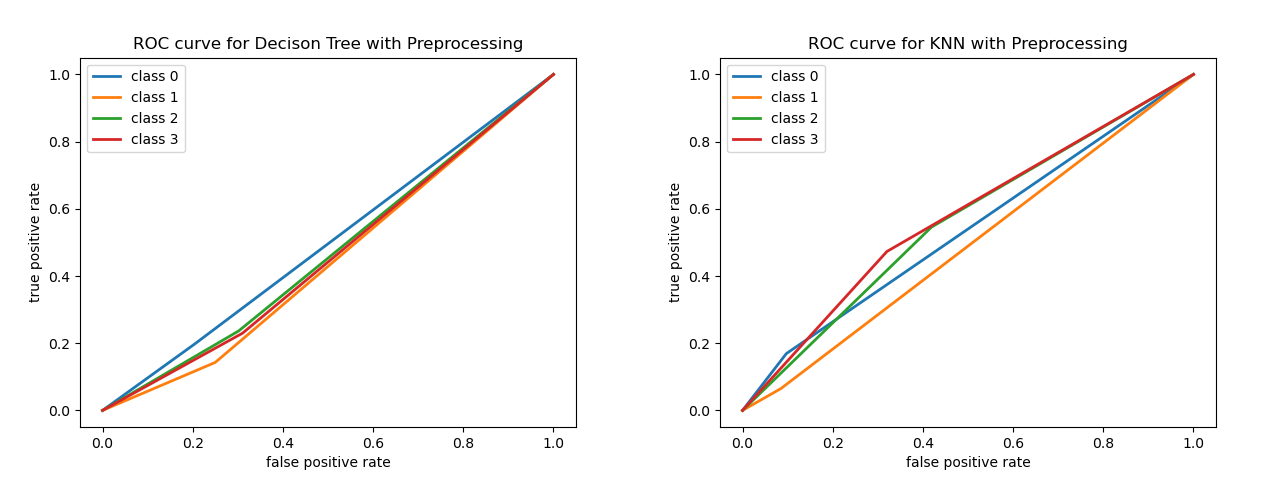
\includegraphics[width=1\columnwidth]{figures/ROC curve DT preprocROC KNN preproc.png}
    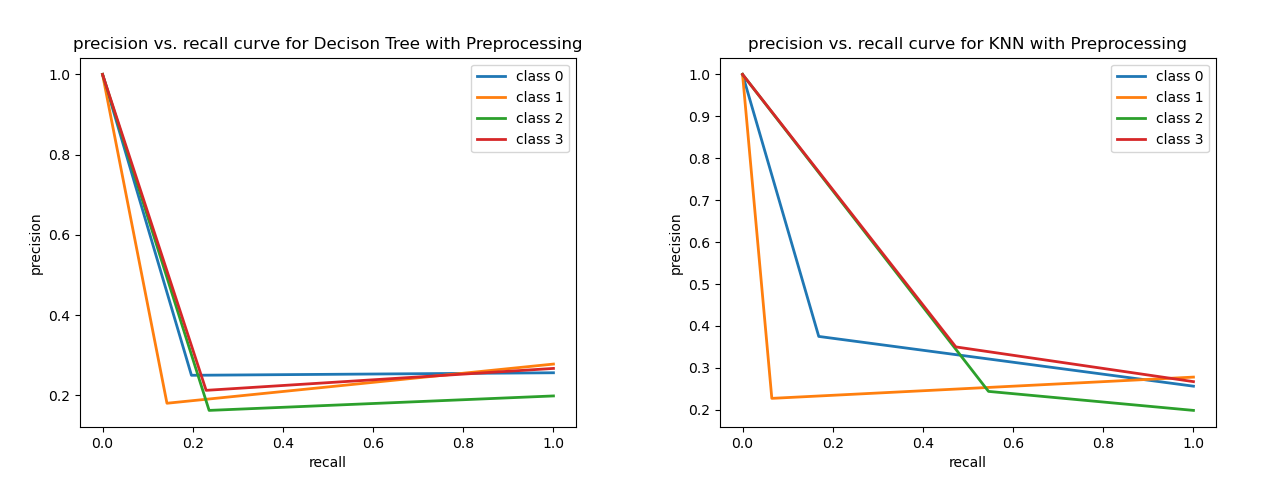
\includegraphics[width=1\columnwidth]{figures/DT Precision vs Recall PreprocPrecision vs Recall KNN preproc.png}
    \caption{ROC curves and Precision vs Recall curves}
    \label{fig:Roc curves}
\end{figure}

Si può osservare senza dubbio che le Roc curves hanno un andamento rappresentativo delle prestazioni riportate a tab. \ref{tab:Performance_Modelli}. Infatti una ROC curve che partendo dall'origine arriva alle coordinate (1,1) indicherebbe che il classificatore è perfetto, ovvero predice in modo esatto le classi. In realtà le immagini sopra mostrate, indicano il contrario per quanto riguarda sopratutto il Decision tree. Infatti la prima classe, la 0, ovvero quella corrispondente alla Portal fibrosis, viene rappresentata con una retta con pendenza a 45 gradi. Ciò significa che il classificatore diventa un classificatore casuale. Al contempo nella ROC curve del KNN sembra esserci un buon risultato di predizione, anche se la classe 1, ovvero "few septa", sembra essere predetta anch'essa casualmente.
Questo tipo di osservazione, si può fare attraverso anche un'altra metrica, chiamata \textbf{AUC}, ovvero Area Under the Curve. Quest'area è proprio l'area sottesa alla curva ROC, il cui valore è compreso tra 0 e 1. Come evidenziato prima, una retta che parte dall'origine (0,0) e finisce nel "top-right corner" (1,1) di questo grafico, avrà come area sottesa 0.5. Tale valore corrisponde appunto ad un classificatore casuale.
\clearpage
\subsection{Prestazioni}
Vengono riportati anche i tempi di processing dei modelli con e senza preprocessing.
\begin{table}[ht]
\centering
\begin{tabular}{@{}lcccll@{}}
\toprule
 & \multicolumn{1}{l}{}                                        & \multicolumn{4}{c}{\textbf{}}                                         \\ \midrule
\multicolumn{1}{|l|}{}                                            & \multicolumn{1}{c|}{}                                       & \multicolumn{4}{c|}{\textit{Processing Time (secs)}}                  \\ \midrule
\multicolumn{1}{|l|}{\multirow{4}{*}{\textbf{For KNN}}}           & \multicolumn{1}{c|}{With Preprocessing}                     & \multicolumn{4}{c|}{0.01197}                                          \\ \cmidrule(l){2-6} 
\multicolumn{1}{|l|}{}                                            & \multicolumn{1}{c|}{\multirow{3}{*}{Without Preprocessing}} & \multicolumn{4}{c|}{\multirow{3}{*}{0.016998}}                        \\
\multicolumn{1}{|l|}{}                                            & \multicolumn{1}{c|}{}                                       & \multicolumn{4}{c|}{}                                                 \\
\multicolumn{1}{|l|}{}                                            & \multicolumn{1}{c|}{}                                       & \multicolumn{4}{c|}{}                                                 \\ \midrule
                                                                  &                                                             &  &                      & \multicolumn{1}{c}{} & \multicolumn{1}{c}{} \\ \midrule
\multicolumn{1}{|l|}{\multirow{5}{*}{\textbf{For Decision Tree}}} & \multicolumn{1}{c|}{With Preprocessing}                     & \multicolumn{4}{c|}{0.00090}                                          \\ \cmidrule(l){2-6} 
\multicolumn{1}{|l|}{}                                            & \multicolumn{1}{c|}{\multirow{3}{*}{Without Preprocessing}} & \multicolumn{4}{c|}{\multirow{3}{*}{0.00200}}                         \\
\multicolumn{1}{|l|}{}                                            & \multicolumn{1}{c|}{}                                       & \multicolumn{4}{c|}{}                                                 \\
\multicolumn{1}{|l|}{}                                            & \multicolumn{1}{c|}{}                                       & \multicolumn{4}{c|}{}                                                 \\ \cmidrule(l){2-6} 
\multicolumn{1}{|l|}{}                                            & \multicolumn{5}{r|}{}                                                                                                               \\ \midrule
                                                                  & \multicolumn{1}{l}{}                                        &  & \multicolumn{1}{r}{} &                      &                      \\ \bottomrule
\end{tabular}
\end{table}
\newline Si nota chiaramente come gli algoritmi, con il preprocessing, e quindi con minor numero di dati tramite la features selection, ci impieghino sensibilmente meno a predire il risultato. 


\clearpage
\bibliography{bibliography/bibliografia.bib}{}
\bibliographystyle{plain}


\end{document}
